Following \cite{Hirsch}, the DGMPM discretizations of scalar linear advection problems are now written in a finite difference sense. The scheme equations thus obtained are the starting points for von Neumann linear stability analyses. First, the one-dimensional problem is considered and scheme equations of the DGMPM space discretization combined to both forward Euler and RK2 explicit time integrations are derived. Second, the two-dimensional scheme equation is written by using the DGMPM space discretization along with the explicit forward Euler time integration only.

\subsection{One-dimensional stability analysis}
\label{subsec:scheme_equations}
\subsubsection*{Model equation - Space discretization}
We consider the scalar linear advection equation for an arbitrary quantity $q=\rho \bar{q}$ moving at the constant speed $a \in \Rbb^{+*}$ in a homogeneous one-dimensional medium of length $l$:
\begin{equation}
\drond{\bar{q}}{t} + \drond{\bar{f}}{X} = 0 
\end{equation}
with specific flux function $\bar{f} = a\bar{q}$, leading to the quasi-linear form:
\begin{equation}
\drond{\bar{q}}{t} + a\drond{\bar{q}}{X} = 0 \label{eq:scalar_advection}
\end{equation}
Equation \eqref{eq:scalar_advection} is discretized with the discontinuous Galerkin material point method. Thus, the medium is divided with $N_p$ material points arbitrarily distributed in $E$ two-nodes elements of constant length $\Delta X$ (figure~\ref{fig:1Dmesh}). The grid mesh is such that at least one particle lies in every cell during the computation in order to ensure that there is no hole in the bar. Moreover, periodic boundary conditions are considered to simplify the analysis.
\begin{figure}[h!]
  \centering
  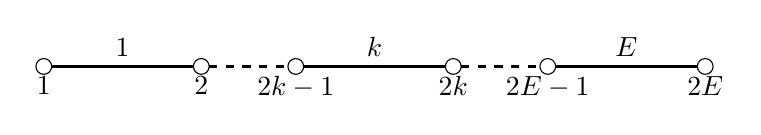
\begin{tikzpicture}
  \draw (2.3,0) circle (0.1) node [below] {$1$};
  \draw (4.3,0) circle (0.1) node [below] {$2$};
  \draw[thick] (2.4,0) -- (4.2,0) node [above,midway] {$1$};
  \draw[thick,dashed] (4.4,0) -- (5.4,0);
  \draw (5.5,0) circle (0.1) node [below] {$2k-1$};
  \draw (7.5,0) circle (0.1) node [below] {$2k$};
  \draw[thick] (5.6,0) -- (7.4,0) node [above,midway] {$k$};
  \draw[thick,dashed] (7.6,0) -- (8.6,0);
  \draw (8.7,0) circle (0.1) node [below] {$2E-1$};
  \draw (10.7,0) circle (0.1) node [below] {$2E$};
  \draw[thick] (8.8,0) -- (10.6,0) node [above,midway] {$E$};
\end{tikzpicture}

  \caption{One-dimensional mesh made of $E$ elements of constant length $\Delta X = \frac{l}{E}$.}\label{fig:1Dmesh}
\end{figure}

Since fields are carried by particles, we seek the scheme equation that gives the solution at a material point for a given time step, with respect to the solutions of other particles at the prior time step. In this section, Latin and Greek symbols are respectively devoted to nodes and material points.
Since we consider here scalar quantities, the information on nodes and particles can be written as subscripts without ambiguity with vector components.
In addition, to make the distinction between fields easier, upper and lower case Latin symbols are used for particles and nodal fields respectively.
Hence, the solution at material point $\alpha$ and time step $n$ reads $\bar{Q}^{n}_\alpha$ whereas that of node $i$ is $\bar{q}^n_i$. Then, the cell containing the particle $\alpha$ will be denoted by $c(\alpha)$ so that the nodes interacting with this particle are $2c(\alpha)-1$ and $2c(\alpha)$. At last, the linear shape functions defined in element $c(\alpha)$ are:
\begin{equation}
S_{2c(\alpha)-1}(X)= \frac{X^{2c(\alpha)} - X}{\Delta X} \qquad S_{2c(\alpha)}(X)= \frac{X -X^{2c(\alpha)-1}}{\Delta X} \qquad X \in \[X^{2c(\alpha)-1},X^{2c(\alpha)}\]
\end{equation}
and $S_{i\alpha}$ or $S_{i,\alpha}$ correspond to the shape function of node $i$ evaluated at the position of the $\alpha$th material point.

\subsubsection*{Scheme equation: Euler time discretization}
The method followed to write the scheme equation is to trace backward the numerical procedure described in section \ref{sec:DGMPM} in order to get an expression of the form \eqref{eq:general_scheme} for the material point $\alpha$:
\begin{equation}
\bar{Q}^{n+1}_\alpha = H\(\bar{Q}^{n}_\beta\) \qquad  \beta=1,..,N_p
\end{equation} 
Quantities at time $t^{n+1}$ are obtained by interpolating nodal solutions of the discrete equation \eqref{eq:DGMPM_discrete} in the cell containing the $\alpha$th particle: 
\begin{equation}
\bar{Q}^{n+1}_\alpha = S_{2c(\alpha)-1,\alpha}\bar{q}_{2c(\alpha)-1}^{n+1} + S_{2c(\alpha),\alpha}\bar{q}_{2c(\alpha)}^{n+1} \label{eq:updated_MP}
\end{equation}
The linear scalar advection equation leads to the interface flux function $\Fc_N =  (aq^*) N $, where
%With the interface fluxes in the case of the linear scalar advection equation $\Fc_N =  (aq^*) N $, in which 
$q^*$ is the stationary solution of Riemann's problem at a cell interface and $N=\pm 1$ the outward unit normal. The discrete form \eqref{eq:DGMPM_discrete} thus reads for both nodes of cell $c(\alpha)$:
\begin{equation}
  \label{eq:nodal_discrete_forms}
  \begin{aligned}
    & \bar{q}_{2c(\alpha)-1}^{n+1}= \bar{q}_{2c(\alpha)-1}^{n} + \frac{\Delta t}{M^L_{2c(\alpha)-1}}\( K_{2c(\alpha)-1,j} a\bar{q}_{j}^{n}- a\rho \bar{q}_{2c(\alpha)-1}^*N_{2c(\alpha)-1} \)\\
    &\bar{q}_{2c(\alpha)}^{n+1}= \bar{q}_{2c(\alpha)}^{n} + \frac{\Delta t}{M^L_{2c(\alpha)}}\( K_{2c(\alpha),j} a\bar{q}_{j}^{n}- a\rho \bar{q}_{2c(\alpha)}^*N_{2c(\alpha)} \)
  \end{aligned}
\end{equation}
where in a one-dimensional grid, the outward unit vectors are $N_{2c(\alpha)-1}=-1$ and $N_{2c(\alpha)}=1$. Discrete equations \eqref{eq:nodal_discrete_forms} are then simplified by first considering that the mass density is defined in a cell as the ratio of total nodal mass and the element volume:
%First, the mass density is defined in a cell as the ratio of total nodal mass and the element volume:
\begin{equation}
  \label{eq:grid_density}
  \rho(X) = \frac{M^L_{2c-1}+M^L_{2c}}{\Delta X} = \frac{\sum_{\mu=1}^{N_p^c} m_\mu}{\Delta X}, \qquad X \in [X^{2c-1},X^{2c}]
\end{equation}
where $N_p^{c}$ is the number of particles in cell $c$ and $m_\mu$, the mass carried by the $\mu$th material point. For homogeneous medium, we further assume that the mass is uniformly distributed between particles so that the previous definition reduces to $\rho = N_p^{c} m^c/\Delta X$, with $m^c$ the mass carried by particles lying in $c$. Second, provided linear shape functions, the lumped mass and the pseudo-stiffness matrices are:
\begin{align}
  & M^L_i = \sum_{\mu=1}^{N_p} S_{i\mu} m_\mu = m^{c(i)} \sum_{\mu=1}^{N_p} S_{i\mu}\\
  & K_{2c(\alpha)-1,j} = \sum_{\mu=1}^{N_p} \drond{S_{2c(\alpha)-1,\mu}}{X} m_\mu S_{j\mu} = -m^{c(i)} \sum_{\mu=1}^{N_p} \frac{ S_{j\mu}}{\Delta X} \\
  & K_{2c(\alpha),j} = \sum_{\mu=1}^{N_p} \drond{S_{2c(\alpha),\mu}}{X} m_\mu S_{j\mu} = m^{c(i)}\sum_{\mu=1}^{N_p} \frac{ S_{j\mu}}{\Delta X} 
\end{align}
The discontinuous approximation basis moreover yields a bloc diagonal pseudo-stiffness matrix so that one can write:
\begin{equation}
  \label{eq:block_diag_K}
  K_{ij} \bar{q}_{j}^{n}= K_{i,2c(i)-1} \bar{q}_{2c(i)-1}^{n}+K_{i,2c(i)} \bar{q}_{2c(i)}^{n}
\end{equation}
Third, a right-going wave (\textit{i.e. $a>0$}) leads to a stationary solution of Riemann problems equals to the state of the upwind node of an interface, that is:
\begin{align}
  & q_{2c(\alpha)-1}^* = \rho \bar{q}^n_{2c(\alpha)-2}=  N_p^{c(\alpha)}\frac{ m^{c(\alpha)}}{\Delta X}\bar{q}^n_{2c(\alpha)-2} \\
  & q_{2c(\alpha)}^* = \rho \bar{q}^n_{2c(\alpha)} =  N_p^{c(\alpha)}\frac{ m^{c(\alpha)}}{\Delta X} \bar{q}^n_{2c(\alpha)} 
\end{align}
Therefore, gathering all the previous considerations, equations \eqref{eq:nodal_discrete_forms} read:
\begin{equation}
  \label{eq:nodal_euler}
  \begin{aligned}
    & \bar{q}_{2c(\alpha)-1}^{n+1}= \bar{q}_{2c(\alpha)-1}^{n} - \frac{a\Delta t}{\Delta X}\( \frac{\sum_{\mu=1}^{N_p^{c(\alpha)}} \[S_{2c(\alpha)-1,\mu}\bar{q}_{2c(\alpha)-1}^{n}+ S_{2c(\alpha),\mu}\bar{q}_{2c(\alpha)}^{n}\] - N_p^{c( \alpha)} \bar{q}^n_{2c(\alpha)-2}}{\sum_{\mu=1}^{N_p^{c(\alpha)}}S_{2c(\alpha)-1,\mu}}\)\\
    &\bar{q}_{2c(\alpha)}^{n+1}= \bar{q}_{2c(\alpha)}^{n} + \frac{a\Delta t}{\Delta X}\( \frac{\sum_{\mu=1}^{N_p^{c(\alpha)}} \[S_{2c(\alpha)-1,\mu}\bar{q}_{2c(\alpha)-1}^{n}+ S_{2c(\alpha),\mu}\bar{q}_{2c(\alpha)}^{n}\]- N_p^{c( \alpha)} \bar{q}^n_{2c(\alpha)}}{\sum_{\mu=1}^{N_p^{c(\alpha)}} S_{2c(\alpha),\mu}} \)
  \end{aligned}
\end{equation}
where the volume fluxes contributions $\sum_{\mu=1}^{N_p^{c}} \[S_{2c-1,\mu}\bar{q}_{2c-1}^{n}+ S_{2c,\mu}\bar{q}_{2c}^{n}\]$ are written for simplicity $f_{c}^{n}$, and Courant number $a\Delta t/\Delta X$ arises. Introduction of those equations in the updated material point solution \eqref{eq:updated_MP} leads after some simplifications to:
\begin{equation}
  \label{eq:euler_before_mapping}
  \begin{split}
    \bar{Q}^{n+1}_\alpha = S_{2c(\alpha)-1,\alpha}q^n_{2c(\alpha)-1}  &+ S_{2c(\alpha),\alpha}\(1-\frac{a\Delta t}{\Delta X}\frac{N_p^{c(\alpha)}}{\sum_\mu S_{2c(\alpha),\mu}}\)q^n_{2c(\alpha)} +N_p^{c(\alpha)}\frac{a\Delta t}{\Delta X} \frac{S_{2c(\alpha)-1,\alpha}}{\sum_\mu S_{2c(\alpha)-1,\mu}}q^n_{2c(\alpha)-2} \\
    & + \frac{a\Delta t}{\Delta X}\(\frac{S_{2c(\alpha),\alpha}}{\sum_\mu S_{2c(\alpha),\mu}}-\frac{S_{2c(\alpha)-1,\alpha}}{\sum_\mu S_{2c(\alpha)-1,\mu}}\)f_{c(\alpha)}^{n}
  \end{split}
\end{equation}

Then, the solutions at nodes and time step $n$ in equation \eqref{eq:euler_before_mapping} result from the projection between particles and the grid \eqref{eq:DGMPM_points2nodes}:
%In equation \eqref{eq:euler_before_mapping} the solutions at nodes result from the convection step \eqref{eq:DGMPM_points2nodes}:
\begin{equation}
\bar{q}^{n}_{i} = \frac{\sum_\beta S_{i\beta}m_\beta \bar{Q}^n_{\beta}}{\sum_\gamma S_{i\gamma}m_\gamma} = \frac{\sum_\beta S_{i\beta} \bar{q}^n_{\beta}}{\sum_\beta S_{i\beta}} \label{eq:stab_mapping}
\end{equation}
In particular, volume fluxes contributions can be written:
\begin{equation}
  f_{c}^{n}=\sum_{\mu=1}^{N_p^{c}}\[S_{2c-1,\mu}\frac{\sum_\beta S_{2c-1,\beta}\bar{q}^n_{\beta}}{\sum_\gamma S_{2c-1,\gamma}}+ S_{2c,\mu}\frac{\sum_\beta S_{2c,\beta} \bar{q}^n_{\beta}}{\sum_\gamma S_{2c,\gamma}} \]=\sum^{N_p}_{\beta=1}\(S_{2c-1,\beta} +S_{2c,\beta} \)\bar{q}^n_{\beta} \label{eq:volume_fluxes_mapped}
\end{equation}
Thus, introduction of mappings \eqref{eq:stab_mapping} and \eqref{eq:volume_fluxes_mapped} in equation \eqref{eq:euler_before_mapping} and permutation of sums over $\beta$ and $i$ lead after some simplifications to the scheme equation:
\begin{equation}
  \begin{split}
    \bar{Q}^{n+1}_\alpha = \sum_{\beta=1}^{N_p} \bar{Q}^{n}_\beta & \left\lbrace \vphantom{\frac{S_{2c(\alpha)-1,\beta}}{\sum_\mu S_{2c(\alpha)-1,\mu}}}S_{2c(\alpha)-1,\alpha}\frac{S_{2c(\alpha)-1,\beta}}{\sum_\mu S_{2c(\alpha)-1,\mu}} + S_{2c(\alpha),\alpha}\frac{S_{2c(\alpha),\beta}}{\sum_\mu S_{2c(\alpha),\mu}} \right. \\
    & -\frac{a\Delta t}{\Delta X}N_p^{c(\alpha)}\frac{S_{2c(\alpha),\alpha}}{\sum_\mu S_{2c(\alpha),\mu}}\frac{S_{2c(\alpha),\beta}}{\sum_\mu S_{2c(\alpha),\mu}}\\
    & + \frac{a\Delta t}{\Delta X}N_p^{c(\alpha)} \frac{S_{2c(\alpha)-1,\alpha}}{\sum_\mu S_{2c(\alpha)-1,\mu}}\frac{S_{2c(\alpha)-2,\beta}}{\sum_\mu S_{2c(\alpha)-2,\mu}} \\
    &\left.+ \frac{a\Delta t}{\Delta X}\[\frac{S_{2c(\alpha),\alpha}}{\sum_\mu S_{2c(\alpha),\mu}}-\frac{S_{2c(\alpha)-1,\alpha}}{\sum_\mu S_{2c(\alpha)-1,\mu}}\]\(S_{2c(\alpha)-1,\beta} +S_{2c(\alpha),\beta}\) \right\rbrace \label{eq:scheme_euler1}
  \end{split}
\end{equation}
Note that the last term of formula \eqref{eq:scheme_euler1} is non-zero if particles $\beta$ and $\alpha$ share the same cell, and in that case the parenthesis is one. Hence, the scheme equation can be rewritten as:
\begin{equation}
  \label{eq:Euler_scheme}
  \begin{split}
    \bar{Q}^{n+1}_\alpha = \sum_{\beta=1}^{N_p} \bar{Q}^{n}_\beta  &\left\lbrace\sum_{i=1}^{2E}S_{i\beta}\frac{S_{i\alpha}}{\sum_\mu S_{i\mu}}  + N_p^{c(\alpha)}\frac{a\Delta t}{\Delta X} \[\frac{S_{2c(\alpha)-1,\alpha}}{\sum_{\mu}  S_{2c(\alpha)-1,\mu}}\frac{S_{2c(\alpha)-2,\beta}}{\sum_{\mu}  S_{2c(\alpha)-2,\mu}}-\frac{S_{2c(\alpha),\alpha}S_{2c(\alpha),\beta}}{\(\sum_{\mu}  S_{2c(\alpha),\mu}\)^2}\]\right.\\
    & + \left.   \frac{a\Delta t}{\Delta X} \[\frac{S_{2c(\beta),\alpha}}{\sum_{\mu}  S_{2c(\beta),\mu}}-\frac{S_{2c(\beta)-1,\alpha}}{\sum_\mu S_{2c(\beta)-1,\mu}}\] \vphantom{\sum_{i=1}^{2E}}\right\rbrace
  \end{split}
\end{equation}
The first (\textit{resp. second}) brackets in equation \eqref{eq:Euler_scheme} involve shape functions that are non zero if material point $\beta$ and $\alpha$ lie in adjacent cells (\textit{resp. the same cell}). Hence, the numerical domain of dependence of the DGMPM for the scalar linear advection equation covers two cells regardless of the number of material points. It is worth noticing that in the particular case of one material point lying in every cells, convective phase \eqref{eq:stab_mapping} simplifies to: $\bar{q}^n_i = \bar{Q}^n_\alpha$ for $c(i)=c(\alpha)$. The mapping therefore amounts to a piece-wise constant reconstruction of the field on the background grid that makes the DGMPM equivalent to the \textit{First Order Upwind (FOU)} method.
However, this no longer holds for other distributions of material points within the computational grid. 

\subsubsection*{Scheme equation: RK2 time discretization}

The discrete system on the grid resulting from the second-order Runge-Kutta time integration consists in the two-stage procedure \eqref{eq:DGMPM_discrete_RK2} which, for the one-dimensional scalar linear advection equation, particularizes at node $i$  as:
\begin{subequations}
  \begin{alignat}{1}
    \label{eq:RK2_stage1}& \bar{q}^{n+1/2}_{i}  =\bar{q}^{n}_{i} + \frac{1}{2}\frac{\Delta t}{M^L_{i}} a \( \sum_{j=1}^{2E} K_{i,j} \bar{q}^n_{j} - q^{*,n}_{i}N_i \) \quad \text{(no sum on $i$)} \\
    \label{eq:RK2_stage2}& \bar{q}^{n+1}_{i}  =\bar{q}^{n}_{i} + \frac{\Delta t}{M^L_{i}} a \( \sum_{j=1}^{2E} K_{i,j} \bar{q}^{n+1/2}_{j} - q^{*,n+1/2}_{i}N_i \) \quad \text{(no sum on $i$)}
  \end{alignat}
\end{subequations}
This procedure can be seen as a recursive use of the Euler scheme \eqref{eq:nodal_euler} with suitable time step sizes. The first stage \eqref{eq:RK2_stage1} yields the intermediate nodal fields in cell $c(\alpha)$:
\begin{equation}
  \label{eq:discrete_RK2_step1}
  \begin{aligned}
    &\bar{q}_{2c(\alpha)-1}^{n+1/2}= \bar{q}_{2c(\alpha)-1}^{n} - \frac{a\Delta t}{2\Delta X}\( \frac{f_{c(\alpha)}^{n} - N_p^{c( \alpha)} \bar{q}^n_{2c(\alpha)-2}}{\sum_{\mu=1}^{N_p^{c(\alpha)}}  S_{2c(\alpha)-1,\mu}}\)\\
    &\bar{q}_{2c(\alpha)}^{n+1/2}= \bar{q}_{2c(\alpha)}^{n} + \frac{a\Delta t}{2\Delta X}\( \frac{f_{c(\alpha)}^{n}- N_p^{c( \alpha)}  \bar{q}^n_{2c(\alpha)}}{\sum_{\mu=1}^{N_p^{c(\alpha)}}  S_{2c(\alpha),\mu}} \)
  \end{aligned}
\end{equation}
and the second \eqref{eq:RK2_stage2} leads to the expression of nodal quantities at the end of the time step:
\begin{equation}
  \label{eq:discrete_RK2_step2}
  \begin{aligned}
    &\bar{q}_{2c(\alpha)-1}^{n+1}= \bar{q}_{2c(\alpha)-1}^{n} - \frac{a\Delta t}{\Delta X}\( \frac{\sum_{\gamma=1}^{N_p^{c(\alpha)}}\[S_{2c(\alpha)-1,\gamma}\bar{q}_{2c(\alpha)-1}^{n+1/2}+ S_{2c(\alpha),\gamma}\bar{q}_{2c(\alpha)}^{n+1/2}\] - N_p^{c( \alpha)} \bar{q}^{n+1/2}_{2c(\alpha)-2}}{\sum_{\mu=1}^{N_p^{c(\alpha)}}  S_{2c(\alpha)-1,\mu}}\)\\
    &\bar{q}_{2c(\alpha)}^{n+1}= \bar{q}_{2c(\alpha)}^{n} + \frac{a\Delta t}{\Delta X}\( \frac{\sum_{\gamma=1}^{N_p^{c(\alpha)}}\[S_{2c(\alpha)-1,\gamma}\bar{q}_{2c(\alpha)-1}^{n+1/2}+ S_{2c(\alpha),\gamma}\bar{q}_{2c(\alpha)}^{n+1/2}\]- N_p^{c( \alpha)}  \bar{q}^{n+1/2}_{2c(\alpha)}}{\sum_{\mu=1}^{N_p^{c(\alpha)}}  S_{2c(\alpha),\mu}} \)
  \end{aligned}
\end{equation}
Then, introduction of the interpolation from nodes to particles \eqref{eq:updated_MP} in equations \eqref{eq:discrete_RK2_step2} leads to the solution at material point $\alpha$ and time step $n+1$:
\begin{equation}
  \begin{split}
    \bar{Q}^{n+1}_\alpha =  &S_{2c(\alpha)-1,\alpha}\bar{q}_{2c(\alpha)-1}^{n} - \(\frac{a\Delta t}{\Delta X}\[S_{2c(\alpha)-1,\alpha} - S_{2c(\alpha),\alpha}\frac{\sum_{\gamma} S_{2c(\alpha)-1,\gamma}}{\sum_{\mu}  S_{2c(\alpha),\mu}}\] \)\bar{q}_{2c(\alpha)-1}^{n+1/2} \\ & +S_{2c(\alpha),\alpha}\bar{q}_{2c(\alpha)}^{n} + \frac{a\Delta t}{\Delta X}\[S_{2c(\alpha),\alpha} - S_{2c(\alpha)-1,\alpha}\frac{\sum_{\gamma} S_{2c(\alpha),\gamma}}{\sum_{\mu}  S_{2c(\alpha)-1,\mu}}- N_p^{c(\alpha)}\frac{S_{2c(\alpha),\alpha}}{\sum_{\mu}  S_{2c(\alpha),\mu}}\] \bar{q}_{2c(\alpha)}^{n+1/2}\\
    &+N_p^{c(\alpha)}\frac{a\Delta t}{\Delta X}\frac{S_{2c(\alpha)-1,\alpha}}{\sum_{\mu}  S_{2c(\alpha)-1,\mu}}\bar{q}_{2c(\alpha)-2}^{n+1/2}
  \end{split}
\end{equation}
Nodal values $q_i^{n+1/2}$ are provided by the first stage of RK2 algorithm and can be substituted in the second stage:
%Note that the volume fluxes contributions $f_c^{n}$ are used in equations \eqref{eq:discrete_RK2_step1} and not in \eqref{eq:discrete_RK2_step2}. Indeed, nodal values $q_i^{n+1/2}$ provided by the first stage of RK2 algorithm are substituted in the second one, it is therefore better to make them appear explicitly. It thus comes:
\begin{equation}
  \begin{split}
    \bar{Q}^{n+1}_\alpha &=  S_{2c(\alpha)-1,\alpha}\bar{q}_{2c(\alpha)-1}^{n} +S_{2c(\alpha),\alpha}\bar{q}_{2c(\alpha)}^{n} \\
    -& \frac{a\Delta t}{\Delta X}\[S_{2c(\alpha)-1,\alpha} - S_{2c(\alpha),\alpha}\frac{\sum_{\mu} S_{2c(\alpha)-1,\mu}}{\sum_{\mu}  S_{2c(\alpha),\mu}}\] \(\bar{q}_{2c(\alpha)-1}^{n} - \frac{a\Delta t}{2\Delta X}\( \frac{f_{c(\alpha)}^{n} - N_p^{c( \alpha)} \bar{q}^n_{2c(\alpha)-2}}{\sum_{\mu}  S_{2c(\alpha)-1,\mu}}\)\) \\
    +& \frac{a\Delta t}{\Delta X}\[S_{2c(\alpha),\alpha}\(1- \frac{N_p^{c(\alpha)}}{\sum_{\mu}  S_{2c(\alpha),\mu}}\) - S_{2c(\alpha)-1,\alpha}\frac{\sum_{\mu} S_{2c(\alpha),\mu}}{\sum_{\mu}  S_{2c(\alpha)-1,\mu}}\] \(\bar{q}_{2c(\alpha)}^{n} + \frac{a\Delta t}{2\Delta X}\( \frac{f_{c(\alpha)}^{n}- N_p^{c( \alpha)}  \bar{q}^n_{2c(\alpha)}}{\sum_{\mu}  S_{2c(\alpha),\mu}} \)\)\\
    +& N_p^{c(\alpha)}\frac{a\Delta t}{\Delta X}\frac{S_{2c(\alpha)-1,\alpha}}{\sum_{\mu}  S_{2c(\alpha)-1,\mu}}\(\bar{q}_{2c(\alpha)-2}^{n} + \frac{a\Delta t}{2\Delta X}\( \frac{f_{c(\alpha)-1}^{n}- N_p^{c( \alpha)}  \bar{q}^n_{2c(\alpha)-2}}{\sum_{\mu}  S_{2c(\alpha)-2,\mu}} \)\) \label{eq:Mp_before_mapping}
  \end{split}
\end{equation}
Note that the solution of the downstream node of the adjacent cell $q^{n+1/2}_{2c(\alpha)-2}$ results from the second equation of the set \eqref{eq:discrete_RK2_step1}. Therefore, by rearranging formula \eqref{eq:Mp_before_mapping} as:
%Note that the second equation of the set \eqref{eq:discrete_RK2_step1} is used for $q^{n+1/2}_{2c(\alpha)-2}$ since it is the downwstream node of the adjacent cell $c(\alpha)-1$. At last, by rearranging formula \eqref{eq:Mp_before_mapping} as:
\begin{equation}
  \begin{split}
    \bar{Q}^{n+1}_\alpha =  &\(S_{2c(\alpha)-1,\alpha} -\frac{a\Delta t}{\Delta X}\[S_{2c(\alpha)-1,\alpha} - S_{2c(\alpha),\alpha}\frac{\sum_{\mu} S_{2c(\alpha)-1,\mu}}{\sum_{\mu}  S_{2c(\alpha),\mu}}\]\)\bar{q}_{2c(\alpha)-1}^{n} \\
    +&\(S_{2c(\alpha),\alpha} + \frac{a\Delta t}{\Delta X}\[S_{2c(\alpha),\alpha}\(1-\frac{N_p^{c(\alpha)}}{\sum_{\mu}  S_{2c(\alpha),\mu}}\) - S_{2c(\alpha)-1,\alpha}\frac{\sum_{\mu} S_{2c(\alpha),\mu}}{\sum_{\mu}  S_{2c(\alpha)-1,\mu}}\]\) \bar{q}_{2c(\alpha)}^{n} \\
    +&\frac{1}{2}\(\frac{a\Delta t}{\Delta X}\)^2\(N_p^{c( \alpha)}\[\frac{S_{2c(\alpha)-1,\alpha}}{\sum_\mu S_{2c(\alpha)-1,\mu}} - \frac{S_{2c(\alpha),\alpha}}{\sum_{\mu}  S_{2c(\alpha),\mu}}\] +S_{2c(\alpha),\alpha} \(\frac{N_p^{c(\alpha)}}{\sum_{\mu}  S_{2c(\alpha),\mu}}\)^2\)\bar{q}_{2c(\alpha)}^{n}\\
    +&N_p^{c( \alpha)}\frac{a\Delta t}{\Delta X}  \[ \frac{S_{2c(\alpha)-1,\alpha}}{\sum_{\mu}  S_{2c(\alpha)-1,\mu}}\(1 -   \frac{a\Delta t}{2\Delta X}\(1+\frac{N_p^{c( \alpha)} }{\sum_{\mu}  S_{2c(\alpha)-2,\mu}} \)\)+\frac{a\Delta t}{2\Delta X} \frac{S_{2c(\alpha),\alpha}}{\sum_{\mu}  S_{2c(\alpha),\mu}}\]\bar{q}^n_{2c(\alpha)-2}\\
    -&\frac{1}{2}\(\frac{a\Delta t}{\Delta X}\)^2 N_p^{c(\alpha)}\frac{S_{2c(\alpha),\alpha}}{\(\sum_{\mu}  S_{2c(\alpha),\mu}\)^2} f_{c(\alpha)}^{n} +\frac{1}{2}\(\frac{a\Delta t}{\Delta X}\)^2N_p^{c(\alpha)}\frac{S_{2c(\alpha)-1,\alpha}}{\sum_{\mu}  S_{2c(\alpha)-1,\mu}}\frac{ f_{c(\alpha)-1}^{n}}{\sum_{\mu}  S_{2c(\alpha)-2,\mu}}
  \end{split}
\end{equation}
the use of mapping equations \eqref{eq:stab_mapping} and \eqref{eq:volume_fluxes_mapped} allows to write:
\begin{equation}
  \begin{split}
    \bar{Q}^{n+1}_\alpha =  &\sum_{\beta} \bar{Q}_\beta^n  \left\lbrace \frac{S_{2c(\alpha)-1,\beta}}{\sum_\mu S_{2c(\alpha)-1,\mu}}\(S_{2c(\alpha)-1,\alpha} -\frac{a\Delta t}{\Delta X}\[S_{2c(\alpha)-1,\alpha} - S_{2c(\alpha),\alpha}\frac{\sum_{\gamma} S_{2c(\alpha)-1,\gamma}}{\sum_{\mu}  S_{2c(\alpha),\mu}}\]\)  \right. \\
    &+\frac{S_{2c(\alpha),\beta}}{\sum_\mu S_{2c(\alpha),\mu}}\(S_{2c(\alpha),\alpha} + \frac{a\Delta t}{\Delta X}\[S_{2c(\alpha),\alpha}\(1-\frac{N_p^{c(\alpha)}}{\sum_{\mu}  S_{2c(\alpha),\mu}}\) - S_{2c(\alpha)-1,\alpha}\frac{\sum_{\gamma} S_{2c(\alpha),\gamma}}{\sum_{\mu}  S_{2c(\alpha)-1,\mu}}\]\)  \\
    &+\frac{S_{2c(\alpha),\beta}}{\sum_\mu S_{2c(\alpha),\mu}}\frac{1}{2}\(\frac{a\Delta t}{\Delta X}\)^2\(N_p^{c( \alpha)}\[\frac{S_{2c(\alpha)-1,\alpha}}{\sum_\mu S_{2c(\alpha)-1,\mu}} - \frac{S_{2c(\alpha),\alpha}}{\sum_{\mu}  S_{2c(\alpha),\mu}}\] +S_{2c(\alpha),\alpha} \(\frac{N_p^{c(\alpha)}}{\sum_{\mu}  S_{2c(\alpha),\mu}}\)^2\)  \\
    &+\frac{N_p^{c( \alpha)} S_{2c(\alpha)-2,\beta}}{\sum_\mu S_{2c(\alpha)-2,\mu}}\frac{a\Delta t}{\Delta X} \[ \frac{S_{2c(\alpha)-1,\alpha}}{\sum_{\mu}  S_{2c(\alpha)-1,\mu}}\(1 -   \frac{a\Delta t}{2\Delta X}\(1+\frac{N_p^{c( \alpha)} }{\sum_{\mu}  S_{2c(\alpha)-2,\mu}} \)\)+\frac{a\Delta t}{2\Delta X} \frac{S_{2c(\alpha),\alpha}}{\sum_{\mu}  S_{2c(\alpha),\mu}}\]\\
    &+\frac{1}{2}\(\frac{a\Delta t}{\Delta X}\)^2 N_p^{c(\alpha)}\left.\( \frac{\[S_{2c(\alpha)-2,\beta} +S_{2c(\alpha)-3,\beta} \]}{\sum_{\mu}  S_{2c(\alpha)-1,\mu}\sum_{\mu}  S_{2c(\alpha)-2,\mu}} S_{2c(\alpha)-1,\alpha}-\frac{\[S_{2c(\alpha)-1,\beta} +S_{2c(\alpha),\beta} \]}{\(\sum_{\mu}  S_{2c(\alpha),\mu}\)^2} S_{2c(\alpha),\alpha}\)  \right\rbrace
  \end{split}
\end{equation}
Once the previous formula is simplified, the one-dimensional scheme equation of the DGMPM with the RK2 time discretization can be written:
\begin{equation}
  \label{eq:RK2_scheme}
  \begin{split}
    \bar{Q}^{n+1}_\alpha =  &\sum_{\beta} \bar{Q}_\beta^n  \left\lbrace \sum_i S_{i\beta}\frac{S_{i\alpha}}{\sum_\mu S_{i\mu}}
      +\frac{a\Delta t}{\Delta X}\[\frac{S_{2c(\beta),\alpha}}{\sum_{\mu}  S_{2c(\beta),\mu}} - \frac{S_{2c(\beta)-1,\alpha}}{\sum_{\mu}  S_{2c(\beta)-1,\mu}}\] \right.\\
    &+\frac{a\Delta t}{\Delta X}N_p^{c( \alpha)}\[\frac{S_{2c(\alpha)-1,\alpha}}{\sum_{\mu}  S_{2c(\alpha)-1,\mu}}\frac{S_{2c(\alpha)-2,\beta}}{\sum_\mu S_{2c(\alpha)-2,\mu}}-\frac{S_{2c(\alpha),\alpha}S_{2c(\alpha),\beta}}{\(\sum_\mu S_{2c(\alpha),\mu}\)^2}\] \\
    &+\frac{1}{2}\(\frac{a\Delta t}{\Delta X}\)^2N_p^{c( \alpha)} \(\frac{S_{2c(\alpha),\beta}}{\sum_\mu S_{2c(\alpha),\mu}}-\frac{S_{2c(\alpha)-2,\beta}}{\sum_\mu S_{2c(\alpha)-2,\mu}}\)\[\frac{S_{2c(\alpha)-1,\alpha}}{\sum_\mu S_{2c(\alpha)-1,\mu}} - \frac{S_{2c(\alpha),\alpha}}{\sum_{\mu}  S_{2c(\alpha),\mu}}\]\\
    &+\frac{1}{2}\(\frac{a\Delta t}{\Delta X}\)^2N_p^{c( \alpha)}\frac{S_{2c(\beta),\alpha}}{\(\sum_{\mu}  S_{2c(\alpha),\mu}\)^2} \[N_p^{c( \alpha)}\frac{S_{2c(\alpha),\beta} }{\sum_\mu S_{2c(\alpha),\mu}}-1\]\\
    &+ \frac{1}{2}\(\frac{a\Delta t}{\Delta X}\)^2\frac{S_{2c(\beta)+1,\alpha}N_p^{c(\alpha)}}{\sum_{\mu}  S_{2c(\alpha)-1,\mu}\sum_{\mu}  S_{2c(\alpha)-2,\mu}} \left.\[ 1 - N_p^{c( \alpha)}\frac{S_{2c(\alpha)-2,\beta} }{\sum_{\mu}  S_{2c(\alpha)-2,\mu}}\] \right\rbrace
    \end{split}
\end{equation}
The three first terms of the latter scheme equation correspond to that obtained for the Euler algorithm \eqref{eq:Euler_scheme} while the second order terms are provided by the two-stage time integration. The brackets in those higher-order corrections vanish when only one point is in each cell of the grid, so that the scheme is, as that of the previous section, equivalent to the FOU method.

\subsubsection*{The von Neumann linear stability analysis}
The scheme equations obtained above are written for simplicity:
\begin{equation}
\bar{Q}^{n+1}_\alpha = \sum_{\beta=1}^{N_p}  D_{\alpha\beta} \bar{Q}^n_{\beta}\label{eq:scheme_Dpi}
\end{equation}
Moreover, the computational domain is repeated periodically by mapping it to the domain $[-l,0]$ so that the solution at material point $\alpha$ and time step $n$ is expanded into a discrete Fourier basis of $2E+1$ harmonics over the domain $X \in \[-l,l\]$:
\begin{equation}
\bar{Q}^{n}_\alpha = \sum_{j=-E}^{E}A_j^n e^{i \alpha k_j \Delta X}
\end{equation}
with $A^n_j$, the magnitude of the $j$th harmonic at time step $n$, $i = \sqrt{-1}$, and $k_j$ a wave number. Introduction of this expansion in equation \eqref{eq:scheme_Dpi} yields:
\begin{equation}
A_j^{n+1} e^{i\alpha k_j \Delta X} = \sum_{\beta=1}^{N_p} A_j^n D_{\alpha\beta}e^{i \beta k_j \Delta X}\quad \forall j=-E,...,E
\end{equation}
The amplification factor between two time steps at a given point is defined as:
\begin{equation}
\frac{A_j^{n+1}}{A_j^n} = \sum_{\beta=1}^{N_p} e^{i (\beta -\alpha)k_j \Delta X} D_{\alpha\beta} \quad \forall j=-E,...,E \label{eq:fourier_expansion}
\end{equation}
A necessary condition to ensure the stability of a numerical scheme is that the amplification factor must be lower than or equal to one in modulus: $\abs{A^{n+1}/A^n} \leq 1$. This upper bound allows to prevent an increasing in error during the computation. For expression \eqref{eq:fourier_expansion}, this leads to:
\begin{equation}
 \abs{\sum_{\beta=1}^{N_p} e^{i (\beta -\alpha)k_j \Delta X} D_{\alpha\beta}} \leq \sum_{\beta=1}^{N_p} \abs{e^{i (\beta -\alpha)k_j \Delta X} D_{\alpha\beta}} = \sum_{\beta=1}^{N_p} \abs{D_{\alpha\beta}} \quad \forall j=-E,...,E
\end{equation}
where the triangle inequality, and the unit modulus of the complex number $e^{\alpha (\beta -\alpha)k_j \Delta X}$ have been used.
Hence, the DGMPM scheme is stable for a given discretization if the Courant number is set so that the following condition is satisfied for all material points:
\begin{equation}
  \label{eq:stability} \sum_{\beta=1}^{N_p} \abs{D_{\alpha\beta}} \leq 1 \quad \forall \: \alpha = 1,...,N_p
\end{equation}
The stability of the scheme is thus ensured by using the lowest CFL number satisfying \eqref{eq:stability}. Note however that the use of the triangle inequality leads to a more severe constraint than that really admissible. As a consequence, the Courant number can be set in practice to higher values than that resulting from the solution of \eqref{eq:stability}. 

%According to scheme equations \eqref{eq:Euler_scheme} or \eqref{eq:RK2_scheme}, such a stability condition can be very hard to find analytically for general discretizations. 
According to scheme equations \eqref{eq:Euler_scheme} or \eqref{eq:RK2_scheme}, the stability condition \eqref{eq:stability} can be very hard to find analytically for general discretizations. 
\begin{table}[h]
  \centering
  \begin{tabular}[ht]{cccccN}
  \hline
  \multicolumn{2}{c}{Number of particles} & Position of $I$th particle in cell $c$ & Euler CFL & RK2 CFL &\\[6pt]
  \hline
  \hline
  (--) &1 &$X^1 \in \[X^{2c-1},X^{2c}\]$  &  1 & 1&\\[8pt]
  \hline
  (i)& 2 & $ X^I= X^{2c-1}+(2I-1)\frac{\Delta X}{4}$ &  0.43 & 1&\\[8pt]
  (ii)& 2 & $X^I= X^{2c-1}+(2I-1)\frac{\Delta X}{4} +\frac{\Delta X}{10} $ &  0.40 & 0.50 &\\[8pt]
  (iii)& 2 & $X^I= X^{2c-1}+(2I-1)\frac{\Delta X}{4} +(I-2)\frac{\Delta X}{10} $ &  0.27 & 1 &\\[8pt]
  (iii)'& 2 & $X^I= X^{2c-1}+(2I-1)\frac{\Delta X}{4} +(I-2)\frac{\Delta X}{4} $ &  0 & 1 &\\[8pt]
  \hline
  (i)& 3 & $ X^I= X^{2c-1}+2I\frac{\Delta X}{8}$ &  0.43 & 1&\\[8pt]
  (ii)& 3 & $X^I= X^{2c-1}+2I\frac{\Delta X}{8} +\frac{\Delta X}{10} $ &  0.40 & 0.50 &\\[8pt]
  (iii)& 3 & $X^I= X^{2c-1}+2I\frac{\Delta X}{8} +(I-2)\frac{\Delta X}{10} $ &  0.27 & 1 &\\[8pt]
  (iii)'& 3 & $X^I= X^{2c-1}+2I\frac{\Delta X}{8} +(I-2)\frac{\Delta X}{4} $ &  0 & 1 &\\[8pt]
  \hline
  (i)& 4 & $ X^I= X^{2c-1}+I\frac{\Delta X}{5}$ &  0.35 & 1&\\[8pt]
  (ii)& 4 & $X^I= X^{2c-1}+I\frac{\Delta X}{5} +\frac{\Delta X}{10} $ &  0.31 & 0.40 &\\[8pt]
  (iii)& 4 & $X^I= X^{2c-1}+I\frac{\Delta X}{5} +\frac{2I-5}{\abs{2I-5}}\frac{\Delta X}{10} $ &  0.18 & 1 &\\[8pt]
  (iii)'& 4 & $X^I= X^{2c-1}+I\frac{\Delta X}{5} +\frac{2I-5}{\abs{2I-5}}\frac{\Delta X}{5} $ &  0 & 1 &\\[8pt]
  \hline
\end{tabular}

%%% Local Variables: 
%%% mode: latex
%%% TeX-master: "../../mainManuscript"
%%% End:
  \caption{DGMPM critical Courant numbers values for Euler or RK2 time integration with respect of the number and positions of material points in a one-dimensional grid. Black circles denote material points while white ones represent grid nodes.}
  \label{tab:CFL_comparison}
\end{table}
Nevertheless, though the infinity of possible material points distributions prevents the explicit derivation of a general stability condition, the optimal CFL number satisfying the equality in \eqref{eq:stability} can be found numerically. Some configurations are studied in table \ref{tab:CFL_comparison} where the critical Courant number resulting from the two time discretizations studied above are compared. Those results have been obtained by using the same particles distribution in every elements of a one-dimensional regular mesh. 
% so that a material point $\alpha$ must lie between the nodes of the cell it belongs to, that is, $X^I \in \[X^{2c-1},X^{2c}\]$. 
First, the DGMPM scheme is stable for all CFL number lower than or equal to one when cells contain one particle only regardless of their positions. This property characterized the FOU method that is retrieved with this discretization. 
Then, when many material points share the same element, several configurations are considered:
\begin{itemize}
\item[(i)] particles are positioned symmetrically with respect to cells centers and regularly spaced in the mesh. This space discretization is referred to as the natural configuration in the following.
\item[(ii)] particles in the natural configuration are all shifted of $u=\Delta X/10$.
\item[(iii)] the same than (ii) with $u$ so that one material point overlaps every left nodes of cells.
\item[(iv)] the same than (iii) for right nodes.
\item[(v)] particles are placed symmetrically with respect to cells centers but not regularly spaced in the mesh. Material points in the left half of cells are shifted of $u_1=-\Delta X/10$ while those in the right half are shifted of $u_2=\Delta X/10$.
\item[(vi)] the same than (v) with the first and last particles overlapping left and right nodes of cells respectively.
\end{itemize}
%RK2 results bad when the upwind material point move to the right
%One can see in table \ref{tab:CFL_comparison} that the RK2 time discretization generally provides better results in terms of CFL number for the particles distributions considered. However, a uniform translation of material points in the mesh leads to a decrease in the Courant number for both time integrations.
First, table \ref{tab:CFL_comparison} shows that the natural configuration leads to the optimal stability bound for the RK2 integrator while the CFL number allowed by using Euler time discretization decreases with increasing number of particles per cell.
Second, moving every points rightward in the mesh (\textit{i.e. cases (ii) and (iv)}) causes a drop in the critical Courant number for both RK2 and Euler algorithms. In particular, stability conditions for more than two particles per cell provided by the RK2 are, in those cases, more restrictive than that of the Euler.
Third, the leftward shifting (\textit{i.e. case (iii)}) leads on the other hand to an improvement of the stability condition for Euler time integration compared to that enabled in the natural configuration. The CFL number provided by RK2 integration also decreases due to the shifting while remaining higher than Euler one.
At last, particles distributions conserving the symmetry with respect to cells centers (\textit{i.e. cases (v) and (vi)}), yield the optimal stability condition for the RK2 integrator while the Euler CFL depends on the spacing between material points. More specifically, Euler algorithm leads to a vanishing CFL for the case (vi), thus preventing any simulation.

% In table \ref{tab:CFL_comparison}, we see that in the natural configuration, RK2 integrator leads to the optimal Courant number whereas the one allowed by using Euler discretization depends on the number of material points in cells. Next, those stability conditions become more restrictive when particles are uniformly translated leftward or rightward in the mesh, whit a more significant decrease in CFL number for a translation in the stream direction (\textit{i.e. cases (ii) and (iv)}). In particular, the RK2 algorithm may yields a lower stability bound than that of Euler approach in situation (iv) with more than two particles per cell.
% % Furthermore the impact of such a translation is more significant in the stream direction (\textit{i.e. cases (ii) and (iv)}) in such a way that the decline in CFL number is bigger than for an inverse stream direction (\textit{i.e. cases (iii)}).
% In the latter situation, the Euler algorithm provides even better results than in the natural configuration. One the other hand, particles distributions that conserve the symmetry with respect to cells centers lead to the optimal stability condition when using the RK2 time integration while the Euler CFL depends on the spacing between material points. More specifically, Euler algorithm leads to a vanishing CFL for the case (vi), thus preventing any simulation.
The distribution of material points, and therefore the resulting quadrature, has an influence on the stability of the scheme. The optimal Courant number can be reached even with the Euler discretization, whereas the classical DGFEM scheme developed in \cite{Chavent_Salzano} is restricted to condition $\Delta t / \Delta X = \Oc(\sqrt{\Delta X})$. This limitation has been addressed by introducing slope limiters in order to remove non-physical oscillations in the vicinity of sharp solutions while providing high-order accuracy in smooth regions \cite{Chavent_Cockburn}. However, the stability of the method was still bounded by $CFL\leq 1/2$ and the scheme was first-order accurate. The use of a second-order Runge-Kutta \cite{DGFEM_CFL} allowed to achieve second-order accuracy of the scheme, but the stability condition then reduced to $CFL\leq1/3$. It is worth noting that space–time DGFEM formulations \cite{ST_DGFEM1,ST_DGFEM2} provided more recently the ability to relax constraints of pure space DGFEM and obtain a critical CFL at 1.

\subsection{Space convergence analysis of the one-dimensional scheme}
\label{sec:convergence}
We now propose to focus numerically on convergence properties of DGMPM schemes for linear elasticity problems in homogeneous solids undergoing one-dimensional stress and strain states so that the bar assumption under small strains holds. The following system of one-dimensional linear scalar advection equations is then considered:  
\begin{equation}
  \label{eq:conv_hyperbolic}
  \drond{}{t} \matrice{v \\ \sigma} -\drond{}{X}\matrice{\frac{1}{\rho}\sigma \\ Ev} = \matrice{0 \\0}
\end{equation}
in a bar of length $l=1\:m$, with Young's modulus $E=2\times10^{11}\: Pa$, and mass density $\rho=7800 \:kg\cdot m^{-3}$. 
The bar is assumed to be initially motionless in a free-stress state, that is: $v(X,0)=0 \:;\:\sigma(X,0)=0 \quad \forall X \in [0,l]$, and subject to the following boundary conditions on its left and right ends respectively:
\begin{equation}
  \label{eq:conv_Bcs}
    \begin{aligned}
    &\sigma(X=0,t) = \tilde{\sigma} \sin\(\frac{0.4\pi t}{T}\)\\
    &\sigma(X=l,t) =0,  \qquad \forall t \in [0,T]
  \end{aligned}
\end{equation}
where $T=\frac{1}{l}\sqrt{\frac{E}{\rho}}$ is the time taken by waves to travel from one end of the bar to the other at the sound speed $c=\sqrt{\frac{E}{\rho}}$. The combination of hyperbolic system \eqref{eq:conv_hyperbolic} and boundary conditions \eqref{eq:conv_Bcs} yields a Picard problem which exact solution is \cite[Ch.2]{Wang}:
\begin{equation}
    \label{eq:exact_solution_convergence}
  \begin{aligned}
    &\sigma(X,t)=\tilde{\sigma} \sin\(\frac{0.4\pi (t-X/c)}{T}\) \\
    & v(X,t)=-\frac{\tilde{\sigma}}{\rho c}\sin\(\frac{0.4\pi (t-X/c)}{T}\), \quad \forall \:X, t \in \[0,l\]\times\[0,T\]
  \end{aligned}
\end{equation}
The continuum system \eqref{eq:conv_hyperbolic} is discretized with both MPM (USF) and DGMPM by using $2^i$ cells ($i=2,3,...,7$) each containing $N_p=2,3,4,8$ regularly spaced material points so that the regular grid size is $\Delta X= l/2^i$. The refinement of the mesh operates on both nodes and particles in such a way that the number and position of material points per cell initially selected is held constant. Configurations involving different numbers of particle per element are studied separately and the CFL number can therefore be set once and for all (optimal for DGMPM, and $0.5$ for the MPM). Numerical solutions are then compared to the exact one \eqref{eq:exact_solution_convergence} according to the relative $L^2$ norm of the error, also referred to as the $L^2$ error $\epsilon$:
\begin{subequations}
  \begin{alignat}{1}
    \label{eq:L2_error_S}
    & \epsilon_\sigma(t) = \(\Delta X \sum_{\alpha=1}^{N_p}\frac{(\sigma_\alpha - \sigma_{\text{exact}}(X_\alpha,t))^2}{\sigma_{\text{exact}}(X_\alpha,t)^2}\)^{\frac{1}{2}} \\
    \label{eq:L2_error_V}
    & \epsilon_v(t) = \(\Delta X \sum_{\alpha=1}^{N_p}\frac{(v_\alpha - v_{\text{exact}}(X_\alpha,t))^2}{v_{\text{exact}}(X_\alpha,t)^2}\)^{\frac{1}{2}}
  \end{alignat}
\end{subequations}
The errors are computed at time $t=0.5 T$ so that no reflection of waves on the right boundary occurs and the stress amplitude is set at $\tilde{\sigma}=4\times 10^4\:Pa$. Figure \ref{fig:convergence_stress} shows the evolution of the $L^2$ errors $\epsilon_\sigma$ with regard to the grid size for the MPM and the DGMPM using Euler and RK2 time discretizations for several number of particles per element. We see that despite the rates of convergence of stress (obtained by means of non-linear least squares fitting and reported in table \ref{tab:accuracy}) are close to one, the DGMPM--Euler and DGMPM--RK2 exhibit lower ones compared to that of the MPM. 
\begin{figure}[h!]
  \centering
  {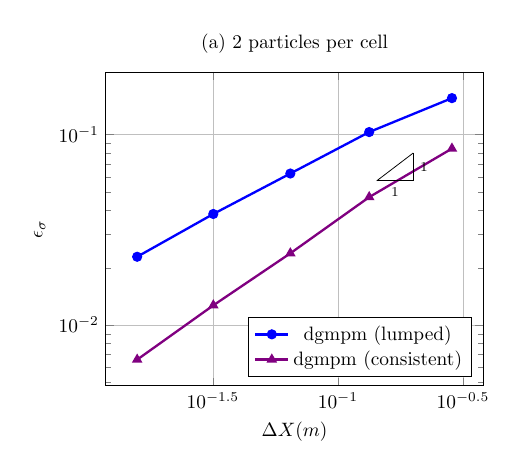
\begin{tikzpicture}[scale=0.7]
\begin{loglogaxis}[xlabel=$\Delta X (m)$,ylabel=$\epsilon_\sigma$,ymajorgrids=true,xmajorgrids=true,legend pos=south east,title={(a) 2 particles per cell}]
\addplot[Blue,very thick,mark=*] coordinates {(0.285714285714,0.155344401413) (0.133333333333,0.103056278416) (0.0645161290323,0.0624467155513) (0.031746031746,0.0383032357895) (0.0157480314961,0.0228383166886) };
\addlegendentry{dgmpm (lumped)}
\addplot[Purple,very thick,mark=triangle*] coordinates {(0.285714285714,0.0844046229439) (0.133333333333,0.0469432859143) (0.0645161290323,0.0238077178296) (0.031746031746,0.0126928564059) (0.0157480314961,0.0065867196308) };
\addlegendentry{dgmpm (consistent)}
\draw (axis cs:0.2,0.08) -- (axis cs:0.2/1.4,0.08/1.4);
\draw (axis cs:0.2,0.08) -- (axis cs:0.2,0.08/1.4) node [midway,right] {\scriptsize 1};
\draw (axis cs:0.2,0.08/1.4) -- (axis cs:0.2/1.4,0.08/1.4) node [midway,below] {\scriptsize 1};
\end{loglogaxis}
\end{tikzpicture}
\phantomsubcaption\label{subfig:convS_2ppc}}
  {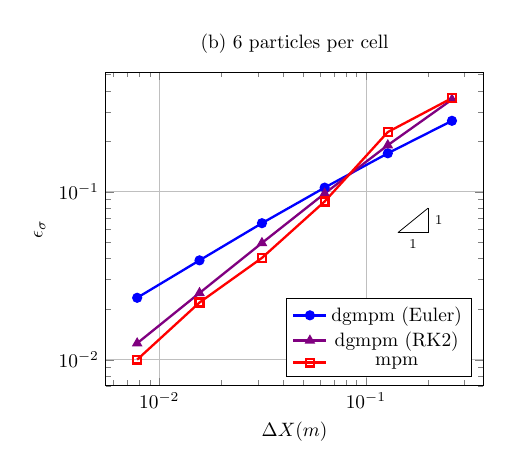
\begin{tikzpicture}[scale=0.7]
\begin{loglogaxis}[xlabel=$\Delta X (m)$,ylabel=$\epsilon_\sigma$,ymajorgrids=true,xmajorgrids=true,legend pos=south east,title={(b) 6 particles per cell}]
\addplot[Blue,very thick,mark=*] coordinates {(0.260869565217,0.264899669611) (0.127659574468,0.169691463046) (0.0631578947368,0.105962740356) (0.0314136125654,0.0650620508673) (0.0156657963446,0.0390852705312) (0.00782268578879,0.0233822325629) };
\addplot[Purple,very thick,mark=triangle*] coordinates {(0.260869565217,0.354522364509) (0.127659574468,0.189702402294) (0.0631578947368,0.0977569338517) (0.0314136125654,0.0495901630096) (0.0156657963446,0.0249717321441) (0.00782268578879,0.0125299028165) };
\addplot[Red,very thick,mark=square] coordinates {(0.260869565217,0.361659189051) (0.127659574468,0.22704913294) (0.0631578947368,0.0875748226303) (0.0314136125654,0.0404157850633) (0.0156657963446,0.0219166787087) (0.00782268578879,0.0100111156173) };
%\addplot[Orange,very thick,mark=+] coordinates {(0.260869565217,0.504029453376) (0.127659574468,0.236059385567) (0.0631578947368,0.123545591795) (0.0314136125654,0.0612427342505) (0.0156657963446,0.0368318555943) (0.00782268578879,0.0193191079163) };
\legend{dgmpm (Euler),dgmpm (RK2),mpm, mpm (pic)}
\draw (axis cs:0.2,0.08) -- (axis cs:0.2/1.4,0.08/1.4);
\draw (axis cs:0.2,0.08) -- (axis cs:0.2,0.08/1.4) node [midway,right] {\scriptsize 1};
\draw (axis cs:0.2,0.08/1.4) -- (axis cs:0.2/1.4,0.08/1.4) node [midway,below] {\scriptsize 1};
\end{loglogaxis}
\end{tikzpicture}
\phantomsubcaption\label{subfig:convS_6ppc}}
  {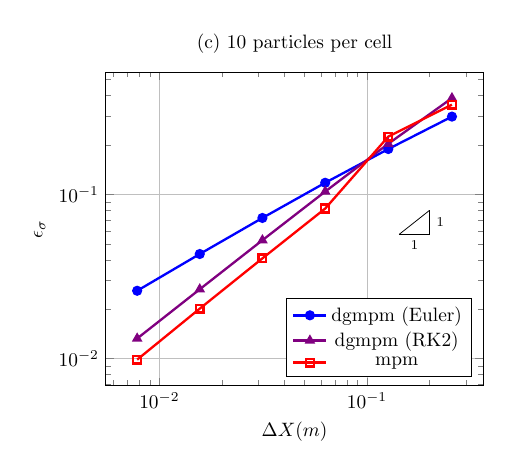
\begin{tikzpicture}[scale=0.7]
\begin{loglogaxis}[xlabel=$\Delta X (m)$,ylabel=$\epsilon_\sigma$,ymajorgrids=true,xmajorgrids=true,legend pos=south east,title={(c) 10 particles per cell}]
\addplot[Blue,very thick,mark=*] coordinates {(0.2564102564102564,0.2977588335733169) (0.12658227848101267,0.18903239674833833) (0.0628930817610063,0.11777400514009143) (0.03134796238244514,0.07191950457145066) (0.015649452269170576,0.043381242893283045) (0.007818608287724786,0.02591311462295878) };
\addlegendentry{dgmpm (Euler)}
\addplot[Purple,very thick,mark=triangle*] coordinates {(0.2564102564102564,0.3858077495889467) (0.12658227848101267,0.2034229849113649) (0.0628930817610063,0.10411628089640804) (0.03134796238244514,0.052639521760385576) (0.015649452269170576,0.026463082691377177) (0.007818608287724786,0.013267145873652044) };
\addlegendentry{dgmpm (RK2)}
\addplot[Red,very thick,mark=square] coordinates {(0.2564102564102564,0.35196127498700136) (0.12658227848101267,0.224972282877443) (0.0628930817610063,0.0820704069820766) (0.03134796238244514,0.04080967339482086) (0.015649452269170576,0.020172859982993875) (0.007818608287724786,0.009867818942546696) };
\addlegendentry{mpm}
\draw (axis cs:0.2,0.08) -- (axis cs:0.2/1.4,0.08/1.4);
\draw (axis cs:0.2,0.08) -- (axis cs:0.2,0.08/1.4) node [midway,right] {\scriptsize 1};
\draw (axis cs:0.2,0.08/1.4) -- (axis cs:0.2/1.4,0.08/1.4) node [midway,below] {\scriptsize 1};
\end{loglogaxis}
\end{tikzpicture}
\phantomsubcaption\label{subfig:convS_10ppc}}
  {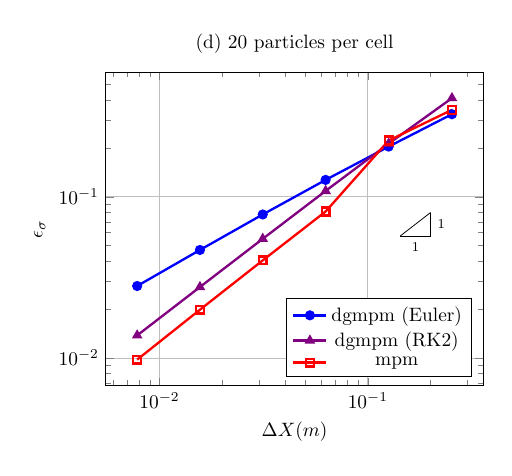
\begin{tikzpicture}[scale=0.7]
\begin{loglogaxis}[xlabel=$\Delta X (m)$,ylabel=$\epsilon_\sigma$,ymajorgrids=true,xmajorgrids=true,legend pos=south east,title={(d) 20 particles per cell}]
\addplot[Blue,very thick,mark=*] coordinates {(0.25316455696202533,0.3259330287835801) (0.1257861635220126,0.20514365080847294) (0.06269592476489028,0.12746685169043193) (0.03129890453834115,0.07779362242457594) (0.015637216575449572,0.04684169163387972) (0.00781555295037124,0.02798669050189462) };
\addlegendentry{dgmpm (Euler)}
\addplot[Purple,very thick,mark=triangle*] coordinates {(0.25316455696202533,0.41013745075143154) (0.1257861635220126,0.21387399252463457) (0.06269592476489028,0.10890822802454231) (0.03129890453834115,0.05492485294977809) (0.015637216575449572,0.02757773169525346) (0.00781555295037124,0.01381741772724311) };
\addlegendentry{dgmpm (RK2)}
\addplot[Red,very thick,mark=square] coordinates {(0.25316455696202533,0.34686018295075766) (0.1257861635220126,0.22381435617895992) (0.06269592476489028,0.08114070769188597) (0.03129890453834115,0.040373135628607865) (0.015637216575449572,0.01994641783412716) (0.00781555295037124,0.009771550248459335) };
\addlegendentry{mpm}
\draw (axis cs:0.2,0.08) -- (axis cs:0.2/1.4,0.08/1.4);
\draw (axis cs:0.2,0.08) -- (axis cs:0.2,0.08/1.4) node [midway,right] {\scriptsize 1};
\draw (axis cs:0.2,0.08/1.4) -- (axis cs:0.2/1.4,0.08/1.4) node [midway,below] {\scriptsize 1};
\end{loglogaxis}
\end{tikzpicture}
\phantomsubcaption\label{subfig:convS_20ppc}}
  \caption{Evolution of the $L^2$ error on stress with regard to the number of particles lying in every cells.}
  \label{fig:convergence_stress}
\end{figure}
\begin{table}[h!]
  \centering
    \begin{tabular}{c|cc|cc|cc|cc}
    \hline
    PPC & \multicolumn{2}{c}{DGMPM--Euler}  \vline & \multicolumn{2}{c}{DGMPM--RK2}\vline  & \multicolumn{2}{c}{MPM} \vline & \multicolumn{2}{c}{MPM--PIC}  \\ [6pt]
    & $\sigma$ & $v$  & $\sigma$ & $v$  & $\sigma$ & $v$ & $\sigma$ & $v$\\ 
    \hline
    \hline
    2 & 0.63 & 0.63 & 0.80 &0.80 & 0.88 & 1.46&0.94& 0.85\\
    6 & 0.66 & 0.66 & 0.91 &0.91 &  0.91&1.62&1.07&0.92\\
    10 & 0.67 & 0.67 & 0.93 &0.93 &0.92&1.62&1.10&0.92\\
    20 & 0.68 & 0.67 & 0.95 &0.95 &0.92&1.61&1.12&0.93\\
    \hline
  \end{tabular}

%%% Local Variables:
%%% mode: latex
%%% TeX-master: "../../mainManuscript"
%%% End:

  \caption{Order of accuracy of MPM and DGMPM with regard to the number of particles per cell}
  \label{tab:accuracy}
\end{table}
Second, an increase in the number of particles per cell provides slightly higher convergence rates, according to table \ref{tab:accuracy}, and shifts DGMPM curves upward as can be seen in figures \ref{fig:convergence_stress}\subref{subfig:convS_2ppc} to \ref{fig:convergence_stress}\subref{subfig:convS_20ppc}. On the other hand, the MPM error curves do not exhibit this behavior as observed in \cite{MPM_BSpline1}. At last, for coarse grids (\textit{i.e. $\Delta X= l/2^i$ for $i \leq 3$}) the DGMPM--Euler leads to the lowest error but its smaller rate of convergence makes it quickly less accurate than the two other methods. Similar behaviors can be seen for the velocity, which convergence curves are depicted in figure \ref{fig:convergence_velocity} for the same discretizations. Again, the DGMPM shows lower rates of convergence than the MPM, and increasing the number of particles per cell leads to more error in DGMPM solutions. The same order of accuracy for velocity and stress resulting from the DGMPM (see table \ref{tab:accuracy}) was expected since the writing of the weak form of system \eqref{eq:conv_hyperbolic} leads to the same approximation for both fields. The MPM is on the other hand, as FEM, characterized by a higher order of convergence for velocity than stress owing to the use of shape functions derivatives for the computation of gradients. Hence, the MPM rate of convergence in terms of velocity is getting closer to two. 

The loss of accuracy in velocity in DGMPM can be explained by the mapping procedure it uses from nodes to particles since FLIP mapping has been introduced in order to reach second-order accuracy \cite{PIC_Nishiguchi}.
Convergence properties of the MPM using PIC projection shown in table \ref{tab:accuracy} and figure \ref{fig:convergence_velocity} confirm the previous remark. Indeed, modifying the way fields are projected from nodes to particles does not affect dramatically the rate of convergence of stress but leads to a significant decrease in velocity accuracy.
\begin{figure}[h!]
  \centering
  {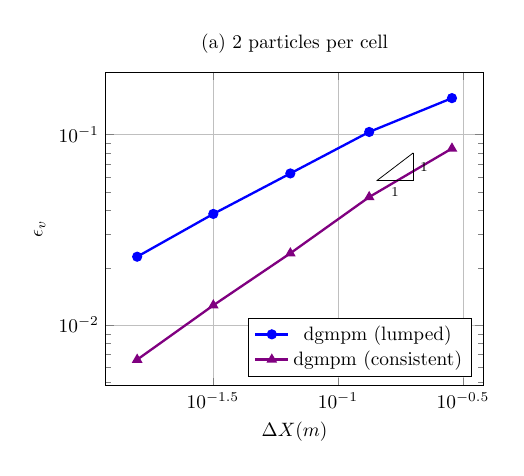
\begin{tikzpicture}[scale=0.7]
\begin{loglogaxis}[xlabel=$\Delta X (m)$,ylabel=$\epsilon_v$,ymajorgrids=true,xmajorgrids=true,legend pos=south east,title={(a) 2 particles per cell}]
\addplot[Blue,very thick,mark=*] coordinates {(0.285714285714,0.155081880585) (0.133333333333,0.103056265942) (0.0645161290323,0.0624467155504) (0.031746031746,0.0383032357895) (0.0157480314961,0.0228383166886) };
\addlegendentry{dgmpm (lumped)}
\addplot[Purple,very thick,mark=triangle*] coordinates {(0.285714285714,0.0844044636359) (0.133333333333,0.0469432859143) (0.0645161290323,0.0238077178296) (0.031746031746,0.0126928564059) (0.0157480314961,0.0065867196308) };
\addlegendentry{dgmpm (consistent)}
\draw (axis cs:0.2,0.08) -- (axis cs:0.2/1.4,0.08/1.4);
\draw (axis cs:0.2,0.08) -- (axis cs:0.2,0.08/1.4) node [midway,right] {\scriptsize 1};
\draw (axis cs:0.2,0.08/1.4) -- (axis cs:0.2/1.4,0.08/1.4) node [midway,below] {\scriptsize 1};
\end{loglogaxis}
\end{tikzpicture}
\phantomsubcaption\label{subfig:convV_2ppc}}
  {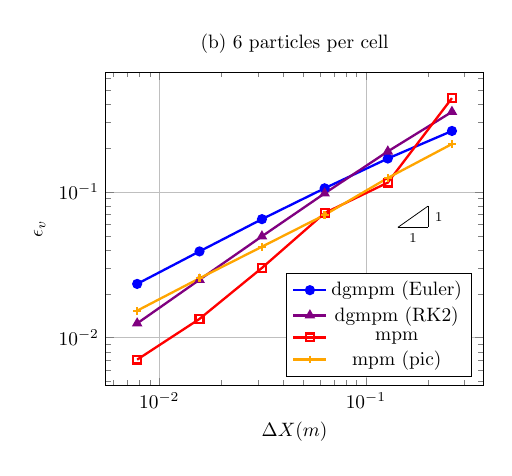
\begin{tikzpicture}[scale=0.7]
\begin{loglogaxis}[xlabel=$\Delta X (m)$,ylabel=$\epsilon_v$,ymajorgrids=true,xmajorgrids=true,legend pos=south east,title={(b) 6 particles per cell}]
\addplot[Blue,very thick,mark=*] coordinates {(0.260869565217,0.262119616463) (0.127659574468,0.169615057945) (0.0631578947368,0.10596257936) (0.0314136125654,0.0650620508656) (0.0156657963446,0.0390852705312) (0.00782268578879,0.0233822325629) };
\addplot[Purple,very thick,mark=triangle*] coordinates {(0.260869565217,0.354522364509) (0.127659574468,0.189702402294) (0.0631578947368,0.0977569338517) (0.0314136125654,0.0495901630096) (0.0156657963446,0.0249717321441) (0.00782268578879,0.0125299028165) };
\addplot[Red,very thick,mark=square] coordinates {(0.260869565217,0.440404482628) (0.127659574468,0.115973424533) (0.0631578947368,0.071649784227) (0.0314136125654,0.0301042119564) (0.0156657963446,0.0134487045496) (0.00782268578879,0.00706618375027) };
\addplot[Orange,very thick,mark=+] coordinates {(0.260869565217,0.2132911803) (0.127659574468,0.124778134951) (0.0631578947368,0.0695253937652) (0.0314136125654,0.0420935361086) (0.0156657963446,0.0255415618466) (0.00782268578879,0.0153163546332) };
\legend{dgmpm (Euler),dgmpm (RK2),mpm, mpm (pic)}
\draw (axis cs:0.2,0.08) -- (axis cs:0.2/1.4,0.08/1.4);
\draw (axis cs:0.2,0.08) -- (axis cs:0.2,0.08/1.4) node [midway,right] {\scriptsize 1};
\draw (axis cs:0.2,0.08/1.4) -- (axis cs:0.2/1.4,0.08/1.4) node [midway,below] {\scriptsize 1};
\end{loglogaxis}
\end{tikzpicture}
\phantomsubcaption\label{subfig:convV_6ppc}}
  {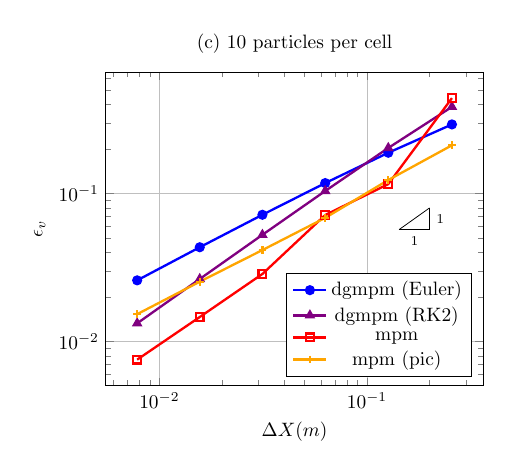
\begin{tikzpicture}[scale=0.7]
\begin{loglogaxis}[xlabel=$\Delta X (m)$,ylabel=$\epsilon_v$,ymajorgrids=true,xmajorgrids=true,legend pos=south east,title={(c) 10 particles per cell}]
\addplot[Blue,very thick,mark=*] coordinates {(0.25641025641,0.293452295348) (0.126582278481,0.188846811163) (0.062893081761,0.117773197736) (0.0313479623824,0.0719195045156) (0.0156494522692,0.0433812428933) (0.00781860828772,0.025913114623) };
\addplot[Purple,very thick,mark=triangle*] coordinates {(0.25641025641,0.385807749589) (0.126582278481,0.203422984911) (0.062893081761,0.104116280896) (0.0313479623824,0.0526395217604) (0.0156494522692,0.0264630826914) (0.00781860828772,0.0132671458737) };
\addplot[Red,very thick,mark=square] coordinates {(0.25641025641,0.441922704379) (0.126582278481,0.115944713051) (0.062893081761,0.0716400384388) (0.0313479623824,0.0286213361273) (0.0156494522692,0.0146450145014) (0.00781860828772,0.00754374417825) };
\addplot[Orange,very thick,mark=+] coordinates {(0.25641025641,0.212130289761) (0.126582278481,0.123526198939) (0.062893081761,0.0685221393014) (0.0313479623824,0.0415170589506) (0.0156494522692,0.02537771007) (0.00781860828772,0.0153081407168) };
\legend{dgmpm (Euler),dgmpm (RK2),mpm, mpm (pic)}
\draw (axis cs:0.2,0.08) -- (axis cs:0.2/1.4,0.08/1.4);
\draw (axis cs:0.2,0.08) -- (axis cs:0.2,0.08/1.4) node [midway,right] {\scriptsize 1};
\draw (axis cs:0.2,0.08/1.4) -- (axis cs:0.2/1.4,0.08/1.4) node [midway,below] {\scriptsize 1};
\end{loglogaxis}
\end{tikzpicture}
\phantomsubcaption\label{subfig:convV_10ppc}}
  {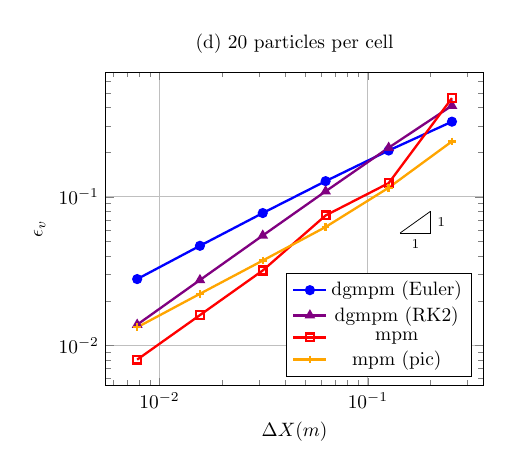
\begin{tikzpicture}[scale=0.7]
\begin{loglogaxis}[xlabel=$\Delta X (m)$,ylabel=$\epsilon_v$,ymajorgrids=true,xmajorgrids=true,legend pos=south east,title={(d) 20 particles per cell}]
\addplot[Blue,very thick,mark=*] coordinates {(0.25316455696202533,0.32008430312967195) (0.1257861635220126,0.20479028039186373) (0.06269592476489028,0.12746427180279027) (0.03129890453834115,0.07779362196760574) (0.015637216575449572,0.04684169163387976) (0.00781555295037124,0.027986690501894642) };
\addlegendentry{dgmpm (Euler)}
\addplot[Purple,very thick,mark=triangle*] coordinates {(0.25316455696202533,0.41013745075143165) (0.1257861635220126,0.21387399252463463) (0.06269592476489028,0.10890822802454243) (0.03129890453834115,0.0549248529497782) (0.015637216575449572,0.027577731695253484) (0.00781555295037124,0.013817417727243226) };
\addlegendentry{dgmpm (RK2)}
\addplot[Red,very thick,mark=square] coordinates {(0.25316455696202533,0.46085003223512083) (0.1257861635220126,0.1236133500299544) (0.06269592476489028,0.07495658911749847) (0.03129890453834115,0.03197022704378847) (0.015637216575449572,0.016023340414579954) (0.00781555295037124,0.008040035849091152) };
\addlegendentry{mpm}
\addplot[Orange,very thick,mark=+] coordinates {(0.25316455696202533,0.2358892840237124) (0.1257861635220126,0.11509251691387613) (0.06269592476489028,0.06267854106060725) (0.03129890453834115,0.0372945293628718) (0.015637216575449572,0.022281125403535065) (0.00781555295037124,0.013263995795214588) };
\addlegendentry{mpm (pic)}
\draw (axis cs:0.2,0.08) -- (axis cs:0.2/1.4,0.08/1.4);
\draw (axis cs:0.2,0.08) -- (axis cs:0.2,0.08/1.4) node [midway,right] {\scriptsize 1};
\draw (axis cs:0.2,0.08/1.4) -- (axis cs:0.2/1.4,0.08/1.4) node [midway,below] {\scriptsize 1};
\end{loglogaxis}
\end{tikzpicture}
\phantomsubcaption\label{subfig:convV_20ppc}}
  \caption{Evolution of the $L^2$ error on velocity with regard to the number of particles lying in every cells.}
  \label{fig:convergence_velocity}
\end{figure}

We now propose to set the Courant number to $0.1$ for the MPM and the DGMPM-Euler in order to compare the accuracy of those first order in time schemes with the same time steps.
\begin{figure}[h!]
  \centering
  {\label{subfig:lowCFL_stress}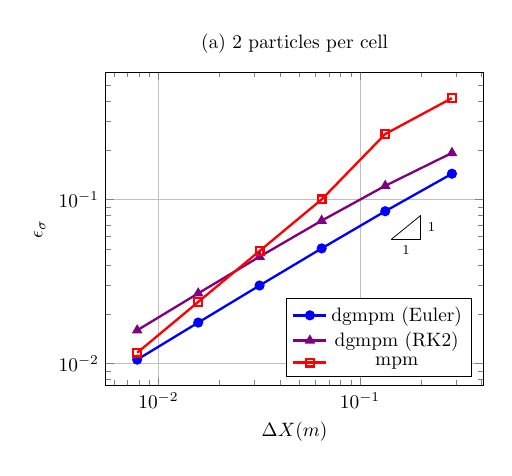
\begin{tikzpicture}[scale=0.7]
\begin{loglogaxis}[xlabel=$\Delta X (m)$,ylabel=$\epsilon_\sigma$,ymajorgrids=true,xmajorgrids=true,legend pos=south east,title={(a) 2 particles per cell}]
\addplot[Blue,very thick,mark=*] coordinates {(0.2857142857142857,0.1436594550802968) (0.13333333333333336,0.08486171615594403) (0.06451612903225806,0.050351766802829157) (0.031746031746031744,0.029913174528173804) (0.015748031496062992,0.017775556941617955) (0.00784313725490196,0.010562958597578517) };
\addlegendentry{dgmpm (Euler)}
\addplot[Purple,very thick,mark=triangle*] coordinates {(0.2857142857142857,0.1924141723102878) (0.13333333333333336,0.12128770020821683) (0.06451612903225806,0.07434664648232299) (0.031746031746031744,0.044831447844707606) (0.015748031496062992,0.026793955118770894) (0.00784313725490196,0.015943520855374583) };
\addlegendentry{dgmpm (RK2)}
\addplot[Red,very thick,mark=square] coordinates {(0.2857142857142857,0.41531074946645796) (0.13333333333333336,0.250867937928352) (0.06451612903225806,0.10016140771414814) (0.031746031746031744,0.04857295290054039) (0.015748031496062992,0.02373902263425921) (0.00784313725490196,0.011630150431372176) };
\addlegendentry{mpm}
\draw (axis cs:0.2,0.08) -- (axis cs:0.2/1.4,0.08/1.4);
\draw (axis cs:0.2,0.08) -- (axis cs:0.2,0.08/1.4) node [midway,right] {\scriptsize 1};
\draw (axis cs:0.2,0.08/1.4) -- (axis cs:0.2/1.4,0.08/1.4) node [midway,below] {\scriptsize 1};
\end{loglogaxis}
\end{tikzpicture}
}
  {\label{subfig:lowCFL_velo}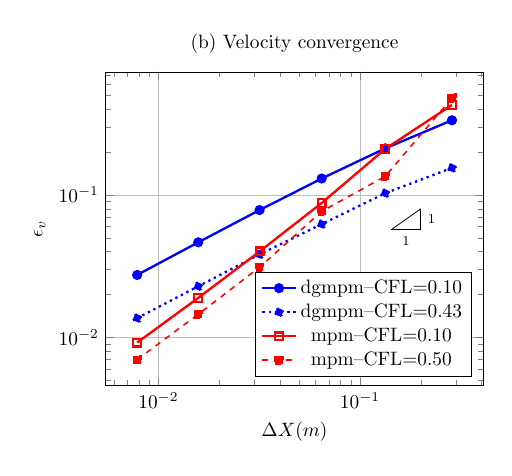
\begin{tikzpicture}[scale=0.7]
\begin{loglogaxis}[xlabel=$\Delta X (m)$,ylabel=$\epsilon_v$,ymajorgrids=true,xmajorgrids=true,legend pos=south east,title={(b) Velocity convergence}]
\addplot[Blue,very thick,mark=*] coordinates {(0.2857142857142857,0.33541409779639897) (0.13333333333333336,0.2128617637917388) (0.06451612903225806,0.13063843103203923) (0.031746031746031744,0.07845857640572454) (0.015748031496062992,0.04654410822285481) (0.00784313725490196,0.027453728586307583) };
\addlegendentry{dgmpm--CFL=0.10}
\addplot[Blue,very thick,dotted,mark=*] coordinates {(0.2857142857142857,0.15508188058471148) (0.13333333333333336,0.10305626594187972) (0.06451612903225806,0.062446715550407435) (0.031746031746031744,0.03830323578950939) (0.015748031496062992,0.022838316688608484) (0.00784313725490196,0.01365358414154964) };
\addlegendentry{dgmpm--CFL=0.43}
% \addplot[Purple,very thick,mark=triangle*] coordinates {(0.2857142857142857,0.33849576213586924) (0.13333333333333336,0.21487150642430616) (0.06451612903225806,0.13190610267495187) (0.031746031746031744,0.07923849924421386) (0.015748031496062992,0.047014965234195974) (0.00784313725490196,0.027734518056277125) };
% \addlegendentry{dgmpm (RK2)}
\addplot[Red,very thick,mark=square] coordinates {(0.2857142857142857,0.4302538204028562) (0.13333333333333336,0.21091773568072011) (0.06451612903225806,0.08791055834347025) (0.031746031746031744,0.04015644182412248) (0.015748031496062992,0.01892979708099774) (0.00784313725490196,0.009194795985585839) };
\addlegendentry{mpm--CFL=0.10}
% \addplot[Orange,very thick,mark=+] coordinates {(0.2857142857142857,0.25515619947095936) (0.13333333333333336,0.13257366926315828) (0.06451612903225806,0.06848518347030894) (0.031746031746031744,0.04006728111884864) (0.015748031496062992,0.02387970823116139) (0.00784313725490196,0.01424585106445727) };
% \addlegendentry{mpm (pic)}
\addplot[Red,thick,dashed,mark=square*] coordinates {(0.2857142857142857,0.47986886216492824) (0.13333333333333336,0.1353831015520096) (0.06451612903225806,0.07678039275069325) (0.031746031746031744,0.03108715264927057) (0.015748031496062992,0.014514861513873035) (0.00784313725490196,0.00697625618426069) };
\addlegendentry{mpm--CFL=0.50}
\draw (axis cs:0.2,0.08) -- (axis cs:0.2/1.4,0.08/1.4);
\draw (axis cs:0.2,0.08) -- (axis cs:0.2,0.08/1.4) node [midway,right] {\scriptsize 1};
\draw (axis cs:0.2,0.08/1.4) -- (axis cs:0.2/1.4,0.08/1.4) node [midway,below] {\scriptsize 1};
\end{loglogaxis}
\end{tikzpicture}
}
  \caption{Evolution of the $L^2$ errors on stress and velocity for two particles per cell. CFL set to 0.1.}
  \label{fig:convergence_lowCFL}
\end{figure}
% \begin{table}[h!]
%   \centering
%     \begin{tabular}{c|cc|cc}%|cc|cc}
    \hline
    PPC & \multicolumn{2}{c}{DGMPM--Euler}  \vline & \multicolumn{2}{c}{MPM}\\%\vline  & \multicolumn{2}{c}{MPM} \vline & \multicolumn{2}{c}{MPM--PIC}  \\ [6pt]
    & $\sigma$ & $v$  & $\sigma$ & $v$  \\%& $\sigma$ & $v$ & $\sigma$ & $v$\\ 
    \hline
    \hline
    2 & 0.66 & 0.66 & 1.00 &1.02 \\%& 0.88 & 1.46&0.94& 0.85\\
    %2 & 0.71 & 0.71 & 0.66 &0.66 \\%& 0.88 & 1.46&0.94& 0.85\\

    
    % 6 & 0.76 & 0.76 & 0.71 &0.71 \\%& 0.91&1.62&1.07&0.92\\
    % 10 & 0.80 & 0.80 & 0.74 &0.74 \\%& 0.92&1.62&1.10&0.92\\
    % 20 & 0.82 & 0.82 & 0.76 &0.76 \\%& 0.92&1.61&1.12&0.93\\
    \hline
  \end{tabular}

%%% Local Variables:
%%% mode: latex
%%% TeX-master: "../../mainManuscript"
%%% End:

%   \caption{Order of accuracy of MPM and DGMPM for two particles per cell and CFL number set to 0.1.}
%   \label{tab:accuracy_low}
% \end{table}
A comparison between the convergence curves obtained for a CFL set to $0.1$ and the previous results (\textit{i.e. figures \ref{fig:convergence_stress} and \ref{fig:convergence_velocity}}) is made in figure \ref{fig:convergence_lowCFL}.
The results first show that the order of accuracy of the DGMPM-Euler is also lower than that of the MPM when the same CFL is used in the methods.
Second, as can be seen in figure \ref{fig:convergence_lowCFL}, the reduction of the time step yields additional error that can be explained by the numerical diffusion introduced in the solutions.
As a consequence, the curves resulting from computations performed with a Courant number set to $0.1$ are above those obtained previously.
However, a lower CFL enables an improvement of the accuracy of the methods. Indeed, the rates of convergence for both velocity and stress are in that case $0.66$ for the DGMPM-Euler, and $1.00$ for the MPM.

Since the DGMPM aims at capturing non-regular solutions (discontinuities), its first-order of convergence is sufficient. Indeed, the achievable accuracy for such solutions is at most one \cite[p.149]{Leveque}. 
Nevertheless, one might be interested in solving problems that involve smooth solutions so that the need of higher-order accuracy arises. Although linear shape functions has been employed so far, the method may handle higher-order approximation by using Legendre polynomials or B-Spline functions for instance (higher-order Lagrange polynomials being to be avoided for moving particles \cite{MPM_BSpline1}). Furthermore, DG features enable to locally increase the approximation order in regions where the solution is smooth. Note however that the particle-based quadrature rule limits the shape functions order one can select since few material points may lead to reduced integration. 
This issue can however be avoided by means of function reconstruction techniques allowing to build a (\textit{linear, quadratic etc.}) function on the grid that is based on the values a field takes at particles locations and which can be evaluated everywhere in a cell. In particular, the use of \textit{moving least squares} \cite{IMPM} or \textit{spline interpolation} \cite{MPM_BSpline1,MPM_BSpline2} within the MPM, enables to evaluate a reconstructed function at Gauss points locations in order to improve the quadrature rule.
Nonetheless, the introduction of such reconstruction techniques in the DGMPM might lead to a restrictive stability condition as it would make the method closer to DGFEM.


Finally, it is worth noticing that only regularly-spaced material points have been considered in the above convergence analysis. An additional means of achieving high-order accuracy can be derived from the following theorem applying to the one-dimensional scalar linear advection equation with $a>0$:
\begin{theorem}[Roe \cite{Toro}]
  \label{th:Roe}
  A numerical scheme of the form:
  \begin{equation}
    \label{eq:scheme_Roe}
    Q^{n+1}_\alpha=\sum_{\beta=-\infty}^{\infty} D_{\beta} Q^{n}_{\alpha+\beta}
  \end{equation}
  is $p$th order accurate ($p\geq 0$) in space and time if and only if:
  \begin{equation}
    \label{eq:Roe_condition}
    \sum_\beta \beta^k D_{\beta} = \(-a\frac{\Delta t}{\Delta X}\)^k \quad 0 \leq k \leq p
  \end{equation}
\end{theorem}
The complexity of scheme equations \eqref{eq:Euler_scheme} and \eqref{eq:RK2_scheme} developed previously, and the lack of such equations for MPM formulations prevent the straightforward calculation of convergence rates. However, one can imagine to build adaption strategies of the set of particles based on theorem \ref{th:Roe}, so that a given order of accuracy is reached. If such a distribution of material point exists, the corresponding Courant number can also be computed, thus ensuring both stability and accuracy of the numerical scheme.


\subsection{Two-dimensional stability analysis}
\subsubsection*{Model equation -- Space discretization}
We now move on to the scalar linear advection equation for an arbitrary quantity $q=\rho \bar{q}$ moving at constant speeds $a,b \in \Rbb^{+*}$ in $X$ and $Y$ directions respectively in a homogeneous two-dimensional medium:
\begin{equation}
  \label{eq:2D_model_equation}
  \drond{\bar{q}}{t} + a\drond{\bar{q}}{X} + b\drond{\bar{q}}{Y}= 0
\end{equation}
Note that the flux functions are in that case $\bar{f}^X = a\bar{q}$ and $\bar{f}^Y = b\bar{q}$. The physical domain $[0,l]\times[0,h]$ is discretized with $N_p$ material points arbitrarily distributed in a Cartesian grid made of $E$ four-node bilinear elements with constant size $\Delta X \times \Delta Y$.
\begin{figure}[h!]
  \centering
  \begin{tikzpicture}
  \draw[thick,->] (-1.5,0.)--(1.5,0.) node [right] {$\xi$};
  \draw[thick,->] (0.,-1.5)--(0.,1.5) node [above] {$\eta$};
  \draw (-1.,-1.0) rectangle (1.,1.);
  \node[above right] at (0.,1.) {$1$};\node[above right] at (0.,-1.) {-$1$};
  \node[above right] at (-1,0.) {-$1$};\node[above right] at (1.,.) {$1$};
  \draw[thick,->] (-.25+5.,0.)--(1.5+5.,0.) node [right] {$X$};
  \draw[thick,->] (0.+5.,-.25)--(0.+5.,1.5) node [above] {$Y$};
  % origin at (+5.,0.)
  \draw (6.,1.) node [below] {$X_1$}-- (8.,1.5) node [below] {$X_2$}-- (9.,4.) node [above] {$X_3$}-- (6.5,3.5) node [above] {$X_4$}-- (6.,1.);
  \fill[black] (8.,3.25) circle (0.05) node [above] {$\vect{X}$};
  \fill[black] (.5,.5) circle (0.05) node [above] {$\vect{\xi}$};
  \draw[->] (8.,3.25) .. controls (6.,3.25) and (1.5,1.5) .. (.5,.5);
\end{tikzpicture}
  
  \caption{Parent and current configuration of a rectangular four-node bilinear element}
  \label{fig:2Dparent}
\end{figure}
With positions of nodes of cell $C$ denoted by $\vect{X}_i^C=\matrice{X^C_i \\ Y_i^C}$ as depicted in figure \ref{fig:2Dparent}, the current location $\vect{X}$ of an arbitrary point in cell $C$ maps to the parent coordinates $(\xi,\eta)$ in the domain $\[-1,1\]\times\[-1,1\]$ according to:
\begin{equation}
  \label{eq:parentCoordinates}
  \begin{aligned}
      &\xi = 2\frac{X-X^C_1}{\Delta X} -1 \quad ; \quad d\xi = 2\frac{dX}{\Delta X} \\
      &\eta = 2\frac{Y-Y^C_1}{\Delta Y} -1 \quad ; \quad d\eta = 2\frac{dY}{\Delta Y} 
  \end{aligned}
\end{equation}
Horizontal and vertical edges lengths are distinguished here in spite of the Cartesian nature of the grid in order to easily extend the following study to rectilinear grids. Again, there is no empty cell inside the physical domain so that no hole is generated, and periodic boundary conditions are considered to simplify the analysis.

\subsubsection*{Two-dimensional scheme equation}
One can imagine to combine the DGMPM discretization with a multi-stage time integration as proposed for one-dimensional problems. The analysis of the DGMPM scheme for two-dimensional problems carried out here however only considers the Euler time discretization.
%As we shall see, the use of the CTU method (see section \ref{subsec:interface_fluxes}) introduces second-order corrections in time within the original DCU approach.
Therefore, the updated solution at material point $\alpha$ is obtained by interpolation of nodal solutions satisfying equation \eqref{eq:2D_model_equation}, discretized as:
\begin{equation}
  \bar{q}_i^{n+1} = \bar{q}_i^n + \frac{\Delta t}{M^L_i} \(K_{ij}^X a\bar{q}_j^n + K_{ij}^Y b\bar{q}_j^n - \hat{f}_i^{*}\) \label{eq:discrete2D}
\end{equation}
so that:
\begin{equation}
  \label{eq:2D_updatedMP}
  \bar{Q}^{n+1}_\alpha = \sum_{i=1}^{4E}S_{i\alpha} \bar{q}_i^{n+1}
\end{equation}
The lumped mass matrix in equation \eqref{eq:discrete2D} has the same expression as in the one-dimensional case that depends on the shape functions of the four-node bilinear element: $M_i^L=\sum_\mu m_\mu S_{i\mu}$. Making use of parent coordinates \eqref{eq:parentCoordinates}, the pseudo-stiffness matrices read:
\begin{equation}
  \begin{aligned}
    & K_{ij}^X = \sum_\beta \drond{S_{i\beta}}{X}m_\beta S_{j\beta}=\frac{2}{\Delta X}\sum_\beta\drond{S_{i\beta}}{\xi}m_\beta S_{j\beta} \\
    &K_{ij}^Y = \sum_\beta\drond{S_{i\beta}}{Y}m_\beta S_{j\beta}=\frac{2}{\Delta Y}\sum_\beta\drond{S_{i\beta}}{\eta}m_\beta S_{j\beta} \\
  \end{aligned}
\end{equation}
As for one-dimensional cases, the homogeneous medium yields the same mass for every particles so that, by writing $\drond{(\bullet)}{\xi}=\partial_\xi(\bullet)$, one gets:
\begin{equation}
  \label{eq:2Dpseudo_stiffness}
  \begin{aligned}
    & \frac{K_{ij}^X}{M_i^L}  =  \frac{2}{\Delta X} \frac{\sum_\lambda\partial_\xi S_{i\lambda}  S_{j\lambda}}{\sum_\gamma  S_{i\gamma}} \\
    & \frac{K_{ij}^Y}{M_i^L} = \frac{2}{\Delta Y} \frac{\sum_\lambda\partial_\eta S_{i\lambda} S_{j\lambda}}{\sum_\gamma S_{i\gamma}}
  \end{aligned}
\end{equation}
The nodal solutions at time $n$ being given by the projection $\bar{q}^{C,n}_i=\frac{\sum_\beta S_{i\beta}\bar{Q}^n_\beta}{\sum_\gamma S_{i\gamma}}$, volume fluxes of the discrete form can be rewritten as:
\begin{equation}
  \label{eq:2Dvolume_fluxes}
  \begin{aligned}
    & a\frac{K_{ij}^X}{M_i^L}\bar{q}^n_j  = \sum_\beta \bar{Q}^n_\beta \frac{2}{\Delta X} \frac{a\sum_\lambda\partial_\xi S_{i\lambda}  \sum_j S_{j\lambda} S_{j\beta}}{\sum_\gamma  S_{i\gamma}\sum_\mu S_{j\mu}}\\
    & b\frac{K_{ij}^Y}{M_i^L}\bar{q}^n_j = \sum_\beta \bar{Q}^n_\beta\frac{2}{\Delta Y}  \frac{b \sum_\lambda\partial_\eta S_{i\lambda}  \sum_j S_{j\lambda} S_{j\beta}}{\sum_\gamma  S_{i\gamma}\sum_\mu S_{j\mu}}
  \end{aligned}
\end{equation}
Then, the nodal interface flux $\hat{f}_i^{*}$ results from the integration of Godunov's fluxes along edges the node belongs to, according to the weak form \eqref{eq:DGMPM_semi_discrete}.
Referring to a quantity defined at an interface by means of parenthesis superscripts, the Godunov's flux corresponding to equation \eqref{eq:2D_model_equation} at interface $(i)$ is:
\begin{equation}
  \label{eq:2d_Godunov_fluxes}
  f^{(i)}= c_n q^{(i)}_U = \underbrace{c_nq^{(i)}_D}_{f_N(q^{(i)}_D)} - \underbrace{c_n (q^{(i)}_D -q^{(i)}_U)}_{A^{+}_{U/D}} 
\end{equation}
where $c_n$ is the speed in the normal direction to the interface (\textit{i.e. b for horizontal and a for vertical edges}). Equation \eqref{eq:2d_Godunov_fluxes} further involves state vectors $q^{(i)}_U$ and $q^{(i)}_D$ obtained by averaging nodal values connected to interface $(i)$ on Upwind and Downwind sides respectively, and the right-going fluctuation $A_{U/D}^+$.
The CTU is adopted by subtracting from fluxes \eqref{eq:2d_Godunov_fluxes} transverse corrections based on those fluctuations according to equation \eqref{eq:transverse_fluctuations}:
\begin{equation}
  \label{eq:2D_transverse_corrections}
  B^+A^+_{U/D}=c_t c_n (q^{(i)}_D -q^{(i)}_U)
\end{equation}
with $c_t$ the speed in the tangent direction to the interface. The final expression of intercell fluxes is hence:
\begin{equation}
  \label{eq:CTU-fluxes}
  f^{(i)}= c_n q^{(i)}_U - c_t c_n (q^{(i)}_D -q^{(i)}_U)
\end{equation}
\begin{figure}[h!]
  \centering
  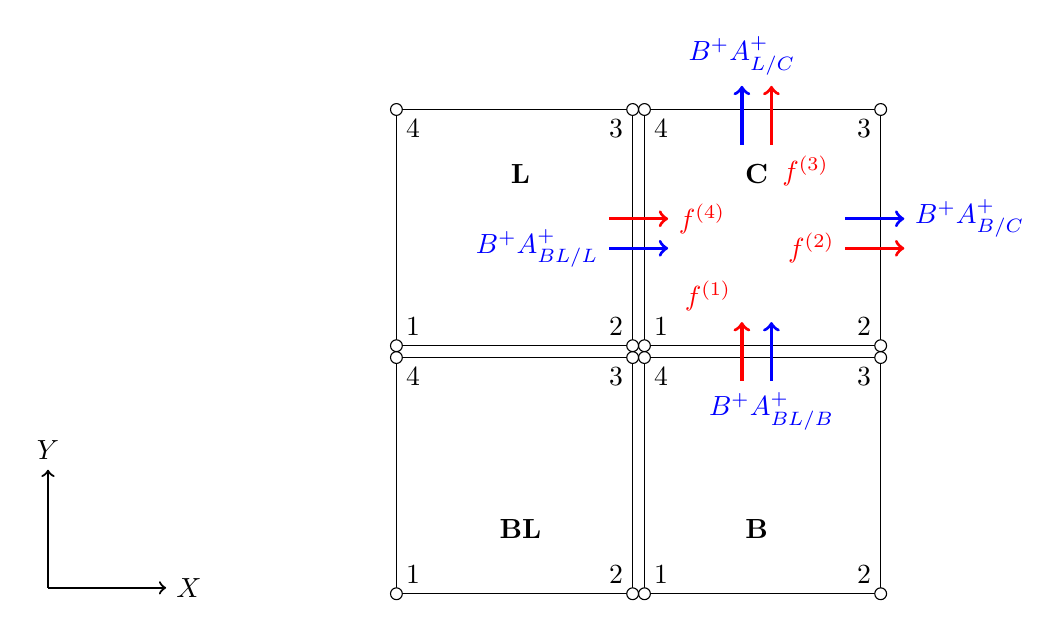
\begin{tikzpicture}[scale=1.5]
  \draw[thick,->] (-3,0.)-- (-2,0.) node[right] {$X$};
  \draw[thick,->] (-3,0.)-- (-3,1.) node[above] {$Y$};

  %% Cells
  \draw (0-0.05,0-0.05) rectangle (2.-0.05,2-0.05);
  \draw (0-0.05,2+0.05) rectangle (2.-0.05,4+0.05);
  \draw (2+0.05,0-0.05) rectangle (4.+0.05,2-0.05);
  \draw (2+0.05,2+0.05) rectangle (4.+0.05,4+0.05);
  %%%%%%%%%%%%%%%%%%%%%
  
  %% Nodes
  \fill[white] (0-0.05,0-0.05) circle (0.05);\fill[white] (2-0.05,2-0.05) circle (0.05);
  \fill[white] (0-0.05,2+0.05) circle (0.05);\fill[white] (2.-0.05,4+0.05) circle (0.05);
  \fill[white] (2+0.05,0-0.05) circle (0.05);\fill[white] (4.+0.05,2-0.05) circle (0.05);
  \fill[white] (2+0.05,2+0.05) circle (0.05);\fill[white] (4.+0.05,4+0.05) circle (0.05);
  \fill[white] (2-0.05,0-0.05) circle (0.05);\fill[white] (4.+0.05,0-0.05) circle (0.05);
  \fill[white] (0-0.05,2-0.05) circle (0.05);\fill[white] (2.+0.05,2-0.05) circle (0.05);
  \fill[white] (2-0.05,2+0.05) circle (0.05);\fill[white] (4.+0.05,2.+0.05) circle (0.05);
  \fill[white] (-0.05,4+0.05) circle (0.05);\fill[white] (2.+0.05,4+0.05) circle (0.05);

  \draw (0-0.05,0-0.05) circle (0.05) node[above right] {$1$};\draw (2-0.05,2-0.05) circle (0.05) node[below left] {$3$};
  \draw (0-0.05,2+0.05) circle (0.05) node[above right] {$1$};\draw (2.-0.05,4+0.05) circle (0.05) node[below left] {$3$};
  \draw (2+0.05,0-0.05) circle (0.05) node[above right] {$1$};\draw (4.+0.05,2-0.05) circle (0.05) node[below left] {$3$};
  \draw (2+0.05,2+0.05) circle (0.05) node[above right] {$1$};\draw (4.+0.05,4+0.05) circle (0.05) node[below left] {$3$};
  \draw (2-0.05,0-0.05) circle (0.05) node[above left] {$2$};\draw (4.+0.05,0-0.05) circle (0.05) node[above left] {$2$};
  \draw (0-0.05,2-0.05) circle (0.05) node[below right] {$4$};\draw (2.+0.05,2-0.05) circle (0.05) node[below right] {$4$};
  \draw (2-0.05,2+0.05) circle (0.05) node[above left] {$2$};\draw (4.+0.05,2.+0.05) circle (0.05) node[above left] {$2$};
  \draw (-0.05,4+0.05) circle (0.05) node[below right] {$4$};\draw (2.+0.05,4+0.05) circle (0.05) node[below right] {$4$};
  %%%%%%%%%%%%%%%%%%%%%%%

  %% Cells names
  \node at (3,3.5) {$\textbf{C}$};
  \node at (1,0.5) {$\textbf{BL}$};
  \node at (3,0.5) {$\textbf{B}$};
  \node at (1,3.5) {$\textbf{L}$};

  %% Transverse corrections
  \draw[->, very thick,Blue] (2.875,3.75) -- (2.875,4.25) node [above] {$B^+A^+_{L/C}$}; % Top
  \draw[->, very thick,Blue] (3.75,3.125) -- (4.25,3.125) node [right] {$B^+A^+_{B/C}$}; % Right
  \draw[<-, very thick,Blue] (3.125,2.25) -- (3.125,1.75) node [below] {$B^+A^+_{BL/B}$}; % Bottom
  \draw[<-, very thick,Blue] (2.25,2.875) -- (1.75,2.875) node [left] {$B^+A^+_{BL/L}$}; % Left

  %% Normal fluxes
  \draw[->, very thick,Red] (3.125,3.75) node [below right] {$f^{(3)}$} -- (3.125,4.25) ; % Top
  \draw[->, very thick,Red] (3.75,2.875) node [left] {$f^{(2)}$}-- (4.25,2.875) ; % Right
  \draw[<-, very thick,Red] (2.875,2.25) node [above left] {$f^{(1)}$}-- (2.875,1.75); % Bottom
  \draw[<-, very thick,Red] (2.25,3.125) node [right] {$f^{(4)}$} -- (1.75,3.125); % Left

  % %% Edges numbers
  % \node[above] at (1,-0.1) {$(1)$};
  % \node[left] at (2,1.) {$(2)$};
  % \node[below] at (1,1.95) {$(3)$};
  % \node[right] at (-0.1,1.) {$(4)$};
\end{tikzpicture}


%%% Local Variables:
%%% mode: latex
%%% TeX-master: "../../mainManuscript"
%%% End:

  \caption{Two-dimensional patch of cells of constant size $\Delta X \times \Delta Y$.}\label{fig:2Dmesh}
\end{figure}
Figure \ref{fig:2Dmesh} shows transverse corrections in the cell $C$ based on fluctuations coming from Bottom ($B$), Left ($L$), Bottom Left ($BL$) neighbor elements. The use of the numbering of interfaces and nodes adopted in figure \ref{fig:2Dmesh} allows the specialization of equation \eqref{eq:CTU-fluxes} to intercell fluxes of cell $C$:
\begin{align}
  & f^{(1)} = b \frac{q_3^{B,n} + q_4^{B,n}}{2} - a b \frac{\Delta t}{2\Delta Y}\(\frac{q_1^{B,n}+q_4^{B,n}}{2}-\frac{q_2^{BL,n}+q_3^{BL,n}}{2}\) \\
  & f^{(2)} = a \frac{q_2^{C,n} + q_3^{C,n}}{2} - a b \frac{\Delta t}{2\Delta X}\(\frac{q_1^{C,n}+q_2^{C,n}}{2}-\frac{q_3^{B,n}+q_4^{B,n}}{2}\) \\
  & f^{(3)} = b \frac{q_3^{C,n} + q_4^{C,n}}{2} - a b \frac{\Delta t}{2\Delta Y}\(\frac{q_1^{C,n}+q_4^{C,n}}{2}-\frac{q_2^{L,n}+q_3^{L,n}}{2}\) \\
  & f^{(4)} = a \frac{q_3^{L,n} + q_4^{L,n}}{2} - a b \frac{\Delta t}{2\Delta X}\(\frac{q_1^{L,n}+q_2^{L,n}}{2}-\frac{q_3^{BL,n}+q_4^{BL,n}}{2}\)
\end{align}
where $q^{C,n}_i= \rho \bar{q}^{C,n}_i$ is the value at time step $n$ and node $i$ of cell $C$. Denoting the number of particles in cell $C$ and the mass they carry by $N_p^C$ and $m^C$ respectively, the mass density reads $\rho = \frac{N_p^{C} m^C}{\Delta X \Delta Y}$. Thus, introduction of the particle fields projection yields the following expressions for interface fluxes:
\begin{align}
  & f^{(1)} = \sum_{\beta=1}^{N_p}\bar{q}_\beta^n\frac{b N^C_p m^C }{2\Delta X \Delta Y} \[  \(\frac{S_{3\beta}^{B} }{\sum_\gamma S_{3\gamma}^{B}} + \frac{S_{4\beta}^{B}}{\sum_\gamma S_{4\gamma}^{B}}\) - a  \frac{\Delta t}{2\Delta Y}\(\frac{S_{1\beta}^{B}}{\sum_\gamma S_{1\gamma}^B} + \frac{S_{4\beta}^{B}}{\sum_\gamma S_{4\gamma}^{B} }-\frac{S_{2\beta}^{BL}}{\sum_\gamma S_{2\gamma}^{BL}} - \frac{S_{3\beta}^{BL}}{\sum_\gamma S_{3\gamma}^{BL}}\) \]\\
  & f^{(2)} = \sum_{\beta=1}^{N_p} \bar{q}_\beta^n\frac{a N^C_p m^C }{2\Delta X \Delta Y} \[  \(\frac{S_{2\beta}^{C}}{\sum_\gamma S_{2\gamma}^{C}} + \frac{S_{3\beta}^{C}}{\sum_\gamma S_{3\gamma}^{C}} \)- b \frac{\Delta t}{2\Delta X}\(\frac{S_{1\beta}^{C}}{\sum_\gamma S_{1\gamma}^{C}} + \frac{S_{2\beta}^{C}}{\sum_\gamma S_{2\gamma}^{C}}-\frac{S_{3\beta}^{B}}{\sum_\gamma S_{3\gamma}^{B}} -\frac{S_{4\beta}^{B}}{\sum_\gamma S_{4\gamma}^{B}}\) \]\\
  & f^{(3)} =\sum_{\beta=1}^{N_p}\bar{q}_\beta^n\frac{b N^C_p m^C}{2\Delta X \Delta Y} \[  \(\frac{S_{3\beta}^{C}}{\sum_\gamma S_{3\gamma}^{C}} + \frac{ S_{4\beta}^{C}}{\sum_\gamma S_{4\gamma}^{C}}\) - a  \frac{\Delta t}{2\Delta Y}\(\frac{S_{1\beta}^{C}}{\sum_\gamma S_{1\gamma}^{C}} + \frac{S_{4\beta}^{C}}{\sum_\gamma S_{4\gamma}^{C}}-\frac{S_{2\beta}^{L}}{\sum_\gamma S_{2\gamma}^{L}} - \frac{S_{3\beta}^{L}}{\sum_\gamma S_{3\gamma}^{L}}\) \]\\
  & f^{(4)} = \sum_{\beta=1}^{N_p}\bar{q}_\beta^n\frac{a N^C_p m^C }{2\Delta X \Delta Y}  \[  \(\frac{S_{3\beta}^{L}}{\sum_\gamma S_{3\gamma}^{L}} + \frac{ S_{4\beta}^{L}}{\sum_\gamma S_{4\gamma}^{L}}\) - b \frac{\Delta t}{2\Delta X}\(\frac{S_{1\beta}^{L}}{\sum_\gamma S_{1\gamma}^{L}} + \frac{S_{2\beta}^{L}}{\sum_\gamma S_{2\gamma}^{L}}-\frac{S_{3\beta}^{BL}}{\sum_\gamma S_{3\gamma}^{BL}} - \frac{S_{4\beta}^{BL}}{\sum_\gamma S_{4\gamma}^{L}}\)\]
\end{align}
written for simplicity:
\begin{equation}
  \label{eq:interface_flux_mapped}
  f^{(i)}=\sum^{N_p}_\beta \bar{Q}_\beta^n \frac{c_n N^C_p m^C}{2\Delta X \Delta Y}\[ \phi_\beta^{(i)} + \phi_\beta^{(i),T} \]
\end{equation}
In the latter expressions, $\phi^{(i)}$ is devoted to normal contributions while $\phi^{(i),T}$ stands for transverse corrections at interface $(i)$. Numerical fluxes considered above are based on normal vectors oriented in the direction of the stream (see figure \ref{fig:2Dmesh}). Nodal interface fluxes on the other hand, as defined in the semi-discrete system:
%Fluxes contribute to nodes through the boundary integrals of the discrete form:
\begin{equation}
  \hat{f}_i^{*} = \int_{\Gamma} S_i(\vect{X}) f^*_N  \: d\Gamma
\end{equation}
are based on the outgoing flux to an element so that $f^{(1)}$ and $f^{(4)}$ must be counted negatively. The integral for cell $C$ is then:
\begin{equation}
  \hat{f}_i^{*} =  -\int_{X^C_1}^{X_2^C} S_i(X,Y^C_{1}) f^{(1)}  dX + \int_{Y^C_2}^{Y_3^C} S_i(X^C_{2},Y) f^{(2)}  dY +\int_{X^C_2}^{X_3^C} S_i(X,Y^C_{3}) f^{(3)}  dX -\int_{Y^C_1}^{Y_4^C} S_i(X^C_{1},Y) f^{(4)}  dY 
\end{equation}
which can be computed analytically by using parent coordinates \eqref{eq:parentCoordinates}:
\begin{subequations}
  \begin{alignat}{4}
    &\hat{f}_1^{*} = -&\frac{1}{2}\[\Delta X f^{(1)} + \Delta Y f^{(4)}\] \quad;\quad &\hat{f}_2^{*} = -&\frac{1}{2}\[\Delta X f^{(1)} - \Delta Y f^{(2)}\]\\
    &\hat{f}_3^{*} =  &\frac{1}{2}\[\Delta X f^{(3)} + \Delta Y f^{(2)}\] \quad;\quad &\hat{f}_4^{*} = &\frac{1}{2}\[\Delta X f^{(3)} - \Delta Y f^{(4)}\]
  \end{alignat}
\end{subequations}
A condensed way of writing those fluxes is adopted by means of the middle point of edge $(j)$ with coordinates $\vect{X}^{(j)}_{1/2}$, at which the shape functions are:
\begin{equation*}
  S_i(\vect{X}^{(j)}_{1/2}) =
  \left\lbrace
  \begin{aligned}
    & \frac{1}{2} \quad \text{if node i belongs to edge (j)} \\
    & 0 \quad \text{otherwise.}
  \end{aligned}
  \right.
\end{equation*}
In addition, components of the outward normal vector to edges $N^{(i)}_X$ and $N^{(i)}_Y$ allows to take into account different signs of intercell fluxes in the Cartesian grid. One thus writes:
\begin{equation}
  \hat{f}_i^{*}= \frac{1}{2}\sum_j^{\text{edges}} 2S_{i}(\vect{X}^{(j)}_{1/2})\(\Delta Y N^{(j)}_X + \Delta X N^{(j)}_Y\) f^{(j)}
\end{equation}
which, combined to equation \eqref{eq:interface_flux_mapped} leads to:
\begin{equation}
  \hat{f}_i^{*}= \sum^{N_p}_\beta \bar{Q}_\beta^n \sum_j^{\text{edges}} S_{i}(\vect{X}^{(j)}_{1/2})\(a\Delta Y N^{(j)}_X + b\Delta X N^{(j)}_Y\)  \frac{ N^C_p m^C}{2\Delta X\Delta Y}\[ \phi_\beta^{(i)} + \phi_\beta^{(i),T} \]
\end{equation}
These terms are divided by the lumped mass matrix in the discrete form:
\begin{equation}
  \label{eq:nodal_fluxes}
  \frac{\hat{f}_i^{*}}{M_i^L}=\sum_\beta \frac{\bar{Q}_\beta^n}{\sum_\mu S_{i\mu}}   \sum_{j=1}^{\text{edges}}\frac{1}{2} S_{i}(\vect{X}^{(j)}_{1/2}) N^C_p m^C \(\frac{aN^{(j)}_X}{\Delta X}  + \frac{bN^{(j)}_Y}{\Delta Y} \) \[\phi_\beta^{(j)} + \phi_\beta^{(j),T}\] 
\end{equation}

At last, gathering the mapping of updated nodal quantities to the particle \eqref{eq:2D_updatedMP}, expressions of volume fluxes \eqref{eq:2Dvolume_fluxes} and intercell ones \eqref{eq:nodal_fluxes}, the updated value at material point $\alpha$ contained in cell $C$ reads:
\begin{equation}
  \label{eq:2Dscheme_equation}
  \begin{split}
    \bar{Q}_\alpha^{n+1}=  \sum_{\beta=1}^{N_p}\bar{Q}_\beta^n\sum_{i=1}^{4E}\frac{S_{i\alpha}}{\sum_\mu S_{i\mu}}  \left\lbrace \vphantom{\sum_{j=1}^{\text{edges}} } \right.& S_{i\beta} +  2  \sum_{j=1}^{4E} \frac{ S_{j\beta}}{\sum_\gamma S_{j\gamma}}\sum_{\lambda=1}^{N_p}S_{j\lambda}\[ a\frac{\Delta t}{\Delta X}\partial_\xi S_{i\lambda}  + b\frac{\Delta t}{\Delta Y} \partial_\eta S_{i\lambda} \] \\ - & \frac{1}{2}\left.\sum_{k=1}^{\text{edges}} S_{i}(\vect{X}^{(k)}_{1/2}) N_p^C \(a\frac{\Delta t}{\Delta X}N^{(j)}_X  + b\frac{\Delta t}{\Delta Y}N^{(j)}_Y \)\[\phi_\beta^{(k)} + \phi_\beta^{(k),T}\] \right\rbrace
  \end{split}
\end{equation}
Recall that transverse contributions $\phi_\beta^{(j),T}$ depend on $\Delta t$, thus providing second-order corrections in the two-dimensional scheme equation \eqref{eq:2Dscheme_equation}, that can also be rewritten as:
\begin{equation}
  \label{eq:2Dscheme_D_alphabeta}
  \bar{Q}_\alpha^{n+1}= \sum_{\beta=1}^{N_p}\bar{Q}_\beta^n D_{\alpha\beta}
\end{equation}

\subsubsection*{The von Neumann linear stability analysis}
Analogously to the one-dimensional case, the solution at a material point can be expanded into a discrete Fourier basis over the domain $\[-l,l\]\times\[-h,h\]$. We consider here a structured distribution of particles made of $N_p=N_p^X\times N_p^Y$ material points so that one can denote the solution at particles by $\bar{Q}_{\alpha\beta}$, where $\alpha$ and $\beta$ are the row and column of material points indices. For one arbitrary Fourier mode, one has \cite[Ch.20]{Leveque}:
\begin{equation}
\bar{Q}^{n}_{\alpha \beta} = A_{jq}^n e^{i (\alpha k_j + \beta k_q)\Delta X}
\end{equation}
where $k_j$ and $k_q$ are wave numbers. Then, the amplification factor reads:
\begin{equation}
\frac{A_{jq}^{n+1}}{A_{jq}^n} =  \sum_{\gamma=1}^{N_p^X}\sum_{\mu=1}^{N_p^Y} e^{i ([\alpha-\gamma]k_j + [\beta-\mu]k_q)\Delta X}D_{\alpha\beta,\gamma\mu}
\end{equation}
with $i=\sqrt{-1}$. The requirement that the absolute value of the amplification factor is lower than or equal to one leads to the following stability condition:
\begin{equation}
\abs{\frac{A_{jq}^{n+1}}{A_{jq}^n}} = \abs{\sum_{\gamma=1}^{N_p^X}\sum_{\mu=1}^{N_p^Y} e^{i ([\alpha-\gamma]k_j + [\beta-\mu]k_q)\Delta X}D_{\alpha\beta,\gamma\mu}} \leq 1 \Leftrightarrow  \sum_{\gamma=1}^{N_p^X}\sum_{\mu=1}^{N_p^Y} \abs{D_{\alpha\beta,\gamma\mu}} \leq 1
\end{equation}
or more simply:
\begin{equation}
\label{eq:2D_stability}
\sum_{\beta=1}^{N_p} \abs{D_{\alpha\beta}} \leq 1 \quad \forall \alpha=1,...,N_p
\end{equation}

Again, the single particle-per-cell discretization leads to a piece-wise constant reconstruction of the field on the computational grid after the projection from material points to nodes, thus providing the first order upwind method. This method is known to be bounded by the stability requirements \cite[Ch.20]{Leveque}:
\begin{subequations}
  \begin{alignat}{2}
    \label{eq:2DCFL_DCU}
    & \abs{a}\frac{\Delta t}{\Delta X} + \abs{b} \frac{\Delta t}{\Delta Y} \leq 1 \qquad &\text{for DCU} \\
    \label{eq:2DCFL_CTU}
    & \max \( \abs{a} \frac{\Delta t}{\Delta X}  , \abs{b} \frac{\Delta t}{\Delta Y}\) \leq 1 \qquad &\text{for CTU}
  \end{alignat}
\end{subequations}

Configurations involving more particles in the computational grid cells are then studied numerically by assuming the same material points distribution in every elements. Furthermore, we consider only regular cells $\Delta Y = \Delta X$ and wave speeds satisfying $a\geq b >0$, so that Courant number reads $a\Delta t/\Delta X$. Coefficients $D_{\alpha \mu}$ depending on both horizontal and vertical wave speeds, the scheme equation \eqref{eq:2Dscheme_D_alphabeta} can be written as a function of the CFL number by means of the speed ratio  $a/b$. Hence, the maximal Courant number satisfying the stability condition \eqref{eq:2D_stability} also depends on the speed ratio.
Evolutions of the CFL numbers corresponding to several distributions of particles in a two-dimensional grid are gathered in tables \ref{tab:2DCFL_comparison_2ppc} and \ref{tab:2DCFL_comparison_4ppc} for the DGMPM scheme using DCU and CTU methods. The first column of this table shows the positions of material points inside cells for discretizations based on $2$ or $4$ particles per element. 

%% 2ppc
The space discretization leading to $2$ particles lying in every cell of the mesh is such that within an element, the two material points are both either on the horizontal axis or on the vertical axis of the cell, corresponding respectively to the results reported in first and second rows of table \ref{tab:2DCFL_comparison_2ppc}. Two situations are then to be distinguished:
\begin{itemize}
\item Material points are regularly-spaced within the grid and placed symmetrically two-by-two with respect to cells centers. Those distributions are drawn in the first column of table \ref{tab:2DCFL_comparison_2ppc} by using blue circles to represent particles.
\item Material points still satisfy symmetry in cells, but are no longer regularly-spaced in the mesh. In that case, particles are drawn with red crosses.
\end{itemize}
\begin{table}[h]
  \centering
  \begin{tabular}[ht]{M{2.5cm}M{5.cm}M{5.cm}N}
  %\setlength\extrarowheight{2.5pt}
  \hline
  Particles in cells & \multicolumn{2}{c}{Critical Courant number $\frac{a\Delta t}{\Delta X}(a/b)$}  & \\[0.5cm]
   &  DCU & CTU & \\
%   & & \multicolumn{2}{c}{$a/b=1$} & \multicolumn{2}{c}{$a/b=10$} & \multicolumn{2}{c}{$a/b=1$} & \multicolumn{2}{c}{$a/b=10$}\\
   % Particles & Position of particles in cell $c$ &  \multicolumn{2}{c}{DCU} & \multicolumn{2}{c}{DCU} \\
  \hline
  \hline
  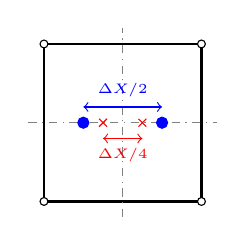
\begin{tikzpicture}[scale=1.]
    \draw[black,thick] (-1.,-1.) rectangle (1.,1.);
    \draw[black!50,dashdotted] (-1.2,0.) -- (1.2,0.0);\draw[black!50,dashdotted] (.0,-1.2) -- (0.,1.2);
    %% nodes
    \fill[white] (-1,-1) circle (0.05);\draw (-1,-1) circle (0.05);
    \fill[white] (1.,-1) circle (0.05);\draw (1,-1) circle (0.05);
    \fill[white] (1,1) circle (0.05);\draw (1,1) circle (0.05);
    \fill[white] (-1.,1) circle (0.05);\draw (-1,1) circle (0.05);
    %% particles
    \draw[Blue,mark=*] plot coordinates {(-0.5,0.)};
    \draw[Blue,mark=*] plot coordinates {(0.5,0.)};
    \draw[Blue,<->] (-0.5,0.2) -- (0.5,0.2) node [midway,above] {\tiny $\Delta X/2$};
    \draw[Red,mark=x] plot coordinates {(-0.25,0.)};
    \draw[Red,mark=x] plot coordinates {(0.25,0.)};
    \draw[Red,<->] (-0.25,-0.2) -- (0.25,-0.2) node [midway,below] {\tiny $\Delta X/4$};
  \end{tikzpicture}  & 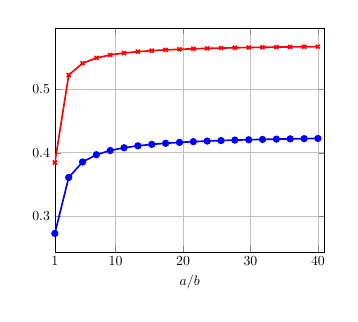
\begin{tikzpicture}[scale=0.5]
\begin{axis}[xlabel=$a/b$,ymajorgrids=true,xmajorgrids=true,xmin=1,xmax=41,xtick={1,10,20,30,40}]
%%%%%%%%%%% NATURAL CONFIGURATION
\addplot[Blue,mark=*,very thick] coordinates {(1.0,0.272727272727) (3.05263157895,0.360995850622) (5.10526315789,0.385430463576) (7.15789473684,0.396887159533) (9.21052631579,0.403535741737) (11.2631578947,0.407878017789) (13.3157894737,0.410936654034) (15.3684210526,0.41320754717) (17.4210526316,0.414960300878) (19.4736842105,0.416354088522) (21.5263157895,0.417488941817) (23.5789473684,0.418430884184) (25.6315789474,0.419225251076) (27.6842105263,0.419904204364) (29.7368421053,0.420491193252) (31.7894736842,0.421003717472) (33.8421052632,0.421455101595) (35.8947368421,0.421855670103) (37.9473684211,0.42221354675) (40.0,0.422535211268) };
%%%%%%%%%%% MODIFIED CONFIGURATION
\addplot[Red,mark=x,very thick] coordinates {(1.0,0.384615384615) (3.05263157895,0.522522522523) (5.10526315789,0.541143654114) (7.15789473684,0.549494949495) (9.21052631579,0.55423594616) (11.2631578947,0.557291666667) (13.3157894737,0.559425096739) (15.3684210526,0.560999039385) (17.4210526316,0.562208067941) (19.4736842105,0.563165905632) (21.5263157895,0.56394346777) (23.5789473684,0.564587271582) (25.6315789474,0.565129097766) (27.6842105263,0.565591397849) (29.7368421053,0.565990483346) (31.7894736842,0.566338490389) (33.8421052632,0.566644635382) (35.8947368421,0.566916043225) (37.9473684211,0.567158308751) (40.0,0.567375886525) };
\end{axis}
\end{tikzpicture}
%%% Local Variables:
%%% mode: latex
%%% TeX-master: "../../mainManuscript"
%%% End:
 & 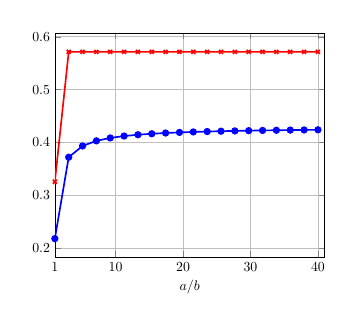
\begin{tikzpicture}[scale=0.5]
\begin{axis}[xlabel=$a/b$,ymajorgrids=true,xmajorgrids=true,xmin=1,xmax=41,xtick={1,10,20,30,40}]
%%%%%%%%%%% NATURAL CONFIGURATION
\addplot[Blue,mark=*,very thick] coordinates {(1.0,0.217751156849) (3.05263157895,0.371899923259) (5.10526315789,0.393212462993) (7.15789473684,0.402887246166) (9.21052631579,0.40840759179) (11.2631578947,0.411975544) (13.3157894737,0.414470966386) (15.3684210526,0.416314181564) (17.4210526316,0.417731290591) (19.4736842105,0.418854723411) (21.5263157895,0.419767189778) (23.5789473684,0.420523008979) (25.6315789474,0.421159327636) (27.6842105263,0.421702408465) (29.7368421053,0.422171344199) (31.7894736842,0.422580347983) (33.8421052632,0.422940218545) (35.8947368421,0.423259307375) (37.9473684211,0.423544174777) (40.0,0.423800045624) };
%%%%%%%%%%% MODIFIED CONFIGURATION
\addplot[Red,mark=x,very thick] coordinates {(1.0,0.325412497399) (3.05263157895,0.571428571428) (5.10526315789,0.571428571429) (7.15789473684,0.571428571429) (9.21052631579,0.57142857143) (11.2631578947,0.571428571429) (13.3157894737,0.571428571429) (15.3684210526,0.571428571429) (17.4210526316,0.571428571429) (19.4736842105,0.571428571429) (21.5263157895,0.571428571429) (23.5789473684,0.571428571429) (25.6315789474,0.571428571429) (27.6842105263,0.571428571429) (29.7368421053,0.571428571429) (31.7894736842,0.571428571429) (33.8421052632,0.571428571429) (35.8947368421,0.571428571429) (37.9473684211,0.571428571429) (40.0,0.571428571429) };
\end{axis}
\end{tikzpicture}
%%% Local Variables:
%%% mode: latex
%%% TeX-master: "../../mainManuscript"
%%% End:
&\\ [3.25cm]%%% SOLUTION
  \hline
  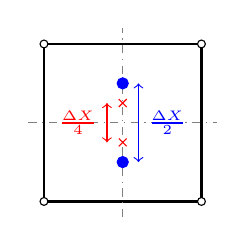
\begin{tikzpicture}[scale=1.]
    \draw[black,thick] (-1.,-1.) rectangle (1.,1.);
    \draw[black!50,dashdotted] (-1.2,0.) -- (1.2,0.0);\draw[black!50,dashdotted] (.0,-1.2) -- (0.,1.2);
    %% nodes
    \fill[white] (-1,-1) circle (0.05);\draw (-1,-1) circle (0.05);
    \fill[white] (1.,-1) circle (0.05);\draw (1,-1) circle (0.05);
    \fill[white] (1,1) circle (0.05);\draw (1,1) circle (0.05);
    \fill[white] (-1.,1) circle (0.05);\draw (-1,1) circle (0.05);
    %% particles
    \draw[Blue,mark=*] plot coordinates {(-0.,-0.5)};
    \draw[Blue,mark=*] plot coordinates {(0.,0.5)};
    \draw[Blue,<->] (0.2,-0.5) -- (0.2,0.5) node [midway,right] {\scriptsize $\frac{\Delta X}{2}$};
    \draw[Red,mark=x] plot coordinates {(0.,-0.25)};
    \draw[Red,mark=x] plot coordinates {(0.,0.25)};
    \draw[Red,<->] (-0.2,-0.25) -- (-0.2,0.25) node [midway,left] {\scriptsize $\frac{\Delta X}{4}$};
  \end{tikzpicture}  & 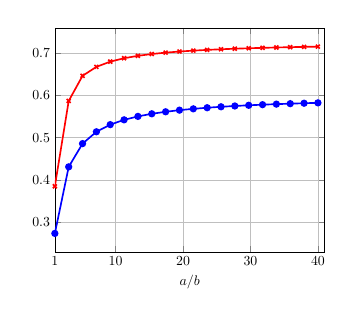
\begin{tikzpicture}[scale=0.5]
\begin{axis}[xlabel=$a/b$,ymajorgrids=true,xmajorgrids=true,xmin=1,xmax=41,xtick={1,10,20,30,40}]
%%%%%%%%%%% NATURAL CONFIGURATION
\addplot[Blue,mark=*,very thick] coordinates {(1.0,0.272727272727) (3.05263157895,0.430693069307) (5.10526315789,0.485809682805) (7.15789473684,0.513853904282) (9.21052631579,0.530839231547) (11.2631578947,0.54222972973) (13.3157894737,0.550398839739) (15.3684210526,0.556543837357) (17.4210526316,0.561334087055) (19.4736842105,0.56517311609) (21.5263157895,0.568318666049) (23.5789473684,0.570943075616) (25.6315789474,0.57316594743) (27.6842105263,0.575072886297) (29.7368421053,0.576726777816) (31.7894736842,0.578174856414) (33.8421052632,0.579453289276) (35.8947368421,0.580590238365) (37.9473684211,0.581607959129) (40.0,0.582524271845) };
%%%%%%%%%%% MODIFIED CONFIGURATION
\addplot[Red,mark=x,very thick] coordinates {(1.0,0.384615384615) (3.05263157895,0.587044534413) (5.10526315789,0.646666666667) (7.15789473684,0.667894413751) (9.21052631579,0.680272108844) (11.2631578947,0.688379573784) (13.3157894737,0.694101508916) (15.3684210526,0.698355754858) (17.4210526316,0.70164281929) (19.4736842105,0.704258862717) (21.5263157895,0.706390328152) (23.5789473684,0.7081604426) (25.6315789474,0.709653916211) (27.6842105263,0.71093090049) (29.7368421053,0.712035286704) (31.7894736842,0.712999852442) (33.8421052632,0.713849569803) (35.8947368421,0.714603798297) (37.9473684211,0.715277777778) (40.0,0.715883668904) };
\end{axis}
\end{tikzpicture}
%%% Local Variables:
%%% mode: latex
%%% TeX-master: "../../mainManuscript"
%%% End:
 & 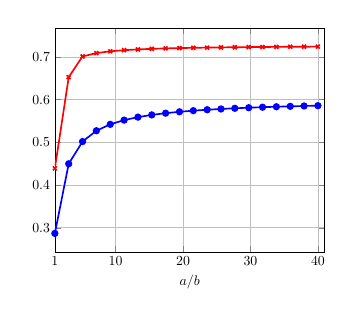
\begin{tikzpicture}[scale=0.5]
\begin{axis}[xlabel=$a/b$,ymajorgrids=true,xmajorgrids=true,xmin=1,xmax=41,xtick={1,10,20,30,40}]
%%%%%%%%%%% NATURAL CONFIGURATION
\addplot[Blue,mark=*,very thick] coordinates {(1.0,0.286705918022) (3.05263157895,0.449716071021) (5.10526315789,0.501782746472) (7.15789473684,0.527153462699) (9.21052631579,0.54213191771) (11.2631578947,0.552009414669) (13.3157894737,0.559009934788) (15.3684210526,0.564229666081) (17.4210526316,0.568271008297) (19.4736842105,0.571492328044) (21.5263157895,0.574120115076) (23.5789473684,0.576304512257) (25.6315789474,0.578148974898) (27.6842105263,0.579727104075) (29.7368421053,0.581092688356) (31.7894736842,0.58228594869) (33.8421052632,0.583337561737) (35.8947368421,0.584271331895) (37.9473684211,0.585106013388) (40.0,0.585856581891) };
%%%%%%%%%%% MODIFIED CONFIGURATION
\addplot[Red,mark=x,very thick] coordinates {(1.0,0.438891399031) (3.05263157895,0.652556925298) (5.10526315789,0.701154248564) (7.15789473684,0.708927502176) (9.21052631579,0.713138668165) (11.2631578947,0.715778473448) (13.3157894737,0.717587786989) (15.3684210526,0.718905133196) (17.4210526316,0.719907103779) (19.4736842105,0.720694821913) (21.5263157895,0.721330359644) (23.5789473684,0.721853926318) (25.6315789474,0.722292713971) (27.6842105263,0.722665770137) (29.7368421053,0.722986834444) (31.7894736842,0.723266066974) (33.8421052632,0.723511142614) (35.8947368421,0.72372796708) (37.9473684211,0.72392115889) (40.0,0.724094381918) };
\end{axis}
\end{tikzpicture}
%%% Local Variables:
%%% mode: latex
%%% TeX-master: "../../mainManuscript"
%%% End:
& \\ [3.25cm] %%% SOLUTION
  \hline
\end{tabular}

%%% Local Variables: 
%%% mode: latex
%%% TeX-master: "../../mainManuscript"
%%% End:
  \caption{Values of critical Courant number $a\frac{\Delta t}{\Delta X}$ for two-dimensional DGMPM scheme using either DCU or CTU with respect to the locations of the $2$ material points lying in every cells as a function of the speeds ratio $a/b$.}
  \label{tab:2DCFL_comparison_2ppc}
\end{table}
First, the results of table \ref{tab:2DCFL_comparison_2ppc} show that the CFL number exhibits a non-linear dependence on speed ratio $a/b$ that asymptotically approach some value which depends on the particles distribution. Second, we see that a reduction of spacing between particles ensuring symmetry between them with respect to cells centers, as for one-dimensional case, yields an increase in the critical Courant number for both DCU and CTU approach. 
Third, whether particles lie on the horizontal axis or the vertical axis of cells has a great influence on the critical Courant number one can expect. Hence, the configurations of the second row of table \ref{tab:2DCFL_comparison_2ppc} yield higher CFL numbers for given speed ratios. It then appears that in order to improve the stability of the scheme, one must use a lower number of material points in the direction of the dominating wave speed than in the perpendicular one. For a Cartesian distribution of particles $N_p^X \times N_p^Y$ this corresponds to $N_p^Y > N_p^X$ if $a>b$, and $N_p^X > N_p^Y$ if $b>a$.
At last, it is worth noticing that the improvement brought by the CTU is much less significant than in the case of one single particle-per-cell discretization for which the Courant number can be set to one according to equations \eqref{eq:2DCFL_DCU} and \eqref{eq:2DCFL_CTU}.

%% 4ppc
We now move on to cases for which grid cells each contains $4$ material points, by considering a square shaped distribution of particles in every elements which centers coincides with cells centroids. This pattern can be contracted or simply translated without change of shape as depicted in the first column of table \ref{tab:2DCFL_comparison_4ppc}. Two configurations are gathered in each row of the table and are distinguished by using either blue circles or red crosses for material points. Again, we observe that the increase in CFL number enabled by the use of the CTU approach is less important that in the case of one particle-per-cell. Next, as for one-dimensional cases and configurations studied in table \ref{tab:2DCFL_comparison_2ppc}, we see that the closer particles are from cell centers, the higher the CFL number is. Finally, it can be seen from the two last rows of table \ref{tab:2DCFL_comparison_4ppc} that the translation of the square of particle inside elements does not have great influence of the evolution of Courant's number with respect to the speed ratio. 
\begin{table}[h!]
  \centering
  \begin{tabular}[ht]{M{2.5cm}M{5.cm}M{5.cm}N}
  %\setlength\extrarowheight{2.5pt}
  \hline
  Particles in cells & \multicolumn{2}{c}{Critical Courant number $\frac{a\Delta t}{\Delta X}(a/b)$}  & \\[0.5cm]
   &  DCU & CTU & \\
%   & & \multicolumn{2}{c}{$a/b=1$} & \multicolumn{2}{c}{$a/b=10$} & \multicolumn{2}{c}{$a/b=1$} & \multicolumn{2}{c}{$a/b=10$}\\
   % Particles & Position of particles in cell $c$ &  \multicolumn{2}{c}{DCU} & \multicolumn{2}{c}{DCU} \\
  \hline
  \hline
  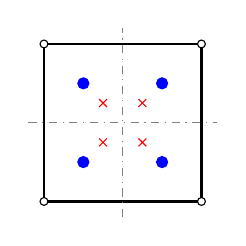
\begin{tikzpicture}[scale=1.]
    \draw[black,thick] (-1.,-1.) rectangle (1.,1.);
    \draw[black!50,dashdotted] (-1.2,0.) -- (1.2,0.0);\draw[black!50,dashdotted] (.0,-1.2) -- (0.,1.2);
    %% nodes
    \fill[white] (-1,-1) circle (0.05);\draw (-1,-1) circle (0.05);
    \fill[white] (1.,-1) circle (0.05);\draw (1,-1) circle (0.05);
    \fill[white] (1,1) circle (0.05);\draw (1,1) circle (0.05);
    \fill[white] (-1.,1) circle (0.05);\draw (-1,1) circle (0.05);
    %% particles
    \draw[Blue,mark=*] plot coordinates {(-0.5,-0.5)};
    \draw[Blue,mark=*] plot coordinates {(0.5,0.5)};
    \draw[Blue,mark=*] plot coordinates {(-0.5,0.5)};
    \draw[Blue,mark=*] plot coordinates {(0.5,-0.5)};
    %\draw[Blue,|-|] (0.5,-0.5) -- (0.5,0.5) node [midway,right] {\scriptsize $\frac{\Delta X}{2}$};
    \draw[Red,mark=x] plot coordinates {(-0.25,-0.25)};
    \draw[Red,mark=x] plot coordinates {(0.25,0.25)};
    \draw[Red,mark=x] plot coordinates {(-0.25,0.25)};
    \draw[Red,mark=x] plot coordinates {(0.25,-0.25)};
    %\draw[Red,|-|] (-0.25,-0.25) -- (-0.25,0.25) node [midway,left] {\scriptsize $\frac{\Delta X}{4}$};
  \end{tikzpicture} & 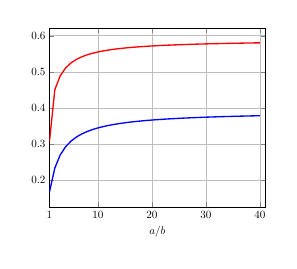
\begin{tikzpicture}[scale=0.4]
\begin{axis}[xlabel=$a/b$,ymajorgrids=true,xmajorgrids=true,xmin=1,xmax=41,xtick={1,10,20,30,40}]
%%%%%%%%%%% NATURAL CONFIGURATION
\addplot[Blue,very thick] coordinates {(1.0,0.166666666667) (2.0,0.233766233766) (3.0,0.27) (4.0,0.292682926829) (5.0,0.308219178082) (6.0,0.319526627219) (7.0,0.328125) (8.0,0.33488372093) (9.0,0.340336134454) (10.0,0.344827586207) (11.0,0.348591549296) (12.0,0.351791530945) (13.0,0.354545454545) (14.0,0.356940509915) (15.0,0.359042553191) (16.0,0.360902255639) (17.0,0.362559241706) (18.0,0.36404494382) (19.0,0.365384615385) (20.0,0.366598778004) (21.0,0.367704280156) (22.0,0.368715083799) (23.0,0.369642857143) (24.0,0.370497427101) (25.0,0.371287128713) (26.0,0.372019077901) (27.0,0.372699386503) (28.0,0.373333333333) (29.0,0.373925501433) (30.0,0.374479889043) (31.0,0.375) (32.0,0.375488917862) (33.0,0.375949367089) (34.0,0.376383763838) (35.0,0.376794258373) (36.0,0.377182770664) (37.0,0.377551020408) (38.0,0.377900552486) (39.0,0.378232758621) (40.0,0.378548895899) };
%%%%%%%%%%% MODIFIED CONFIGURATION
\addplot[Red,very thick] coordinates {(1.0,0.30612244898) (2.0,0.450574712644) (3.0,0.488913525499) (4.0,0.510638297872) (5.0,0.524625267666) (6.0,0.534383520145) (7.0,0.541578947368) (8.0,0.547103977669) (9.0,0.551479783243) (10.0,0.555031149707) (11.0,0.557971014493) (12.0,0.560444797458) (13.0,0.562555195761) (14.0,0.564376799671) (15.0,0.565965092402) (16.0,0.567362199976) (17.0,0.568600682594) (18.0,0.569706103994) (19.0,0.570698814875) (20.0,0.571595217265) (21.0,0.572408677916) (22.0,0.57315019938) (23.0,0.57382892057) (24.0,0.574452495319) (25.0,0.575027382256) (26.0,0.575559069347) (27.0,0.576052249637) (28.0,0.576510960151) (29.0,0.576938692651) (30.0,0.577338482686) (31.0,0.577712981744) (32.0,0.578064516129) (33.0,0.578395135328) (34.0,0.578706652) (35.0,0.579000675219) (36.0,0.579278638279) (37.0,0.579541822056) (38.0,0.579791374747) (39.0,0.580028328612) (40.0,0.58025361425) };
\end{axis}
\end{tikzpicture}
%%% Local Variables:
%%% mode: latex
%%% TeX-master: "../../mainManuscript"
%%% End:
 & 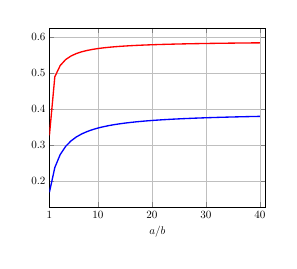
\begin{tikzpicture}[scale=0.4]
\begin{axis}[xlabel=$a/b$,ymajorgrids=true,xmajorgrids=true,xmin=1,xmax=41,xtick={1,10,20,30,40}]
%%%%%%%%%%% NATURAL CONFIGURATION
\addplot[Blue,very thick] coordinates {(1.0,0.167891991267) (2.0,0.236676134687) (3.0,0.272980739363) (4.0,0.295523052838) (5.0,0.31086679909) (6.0,0.321980387453) (7.0,0.330399242911) (8.0,0.336996589796) (9.0,0.342305428681) (10.0,0.346669420492) (11.0,0.350320058356) (12.0,0.353418957124) (13.0,0.356082359353) (14.0,0.358396007915) (15.0,0.360424530234) (16.0,0.362217559503) (17.0,0.363813843724) (18.0,0.36524407401) (19.0,0.366532874772) (20.0,0.367700231858) (21.0,0.368762535467) (22.0,0.369733353839) (23.0,0.370624015434) (24.0,0.371444052722) (25.0,0.372201544487) (26.0,0.372903382721) (27.0,0.373555482814) (28.0,0.374162950599) (29.0,0.374730216246) (30.0,0.375261142441) (31.0,0.375759112422) (32.0,0.376227102125) (33.0,0.376667739677) (34.0,0.377083354767) (35.0,0.377476019835) (36.0,0.37784758462) (37.0,0.378199705293) (38.0,0.378533869127) (39.0,0.378851415496) (40.0,0.379153553806) };
%%%%%%%%%%% MODIFIED CONFIGURATION
\addplot[Red,very thick] coordinates {(1.0,0.326304188278) (2.0,0.489325348197) (3.0,0.520649204857) (4.0,0.537092735424) (5.0,0.547194071957) (6.0,0.554021734434) (7.0,0.558942755592) (8.0,0.56265696686) (9.0,0.565559375666) (10.0,0.567889697418) (11.0,0.56980178835) (12.0,0.571398904651) (13.0,0.572752913461) (14.0,0.573915372853) (15.0,0.57492422974) (16.0,0.575808031925) (17.0,0.57658866765) (18.0,0.577283199978) (19.0,0.577905126649) (20.0,0.578465264862) (21.0,0.578972385091) (22.0,0.579433673213) (23.0,0.579855072848) (24.0,0.580241542647) (25.0,0.580597252178) (26.0,0.580925732862) (27.0,0.581229995544) (28.0,0.581512622996) (29.0,0.58177584338) (30.0,0.582021589074) (31.0,0.58225154418) (32.0,0.582467183146) (33.0,0.58266980241) (34.0,0.582860546471) (35.0,0.583040429512) (36.0,0.583210353437) (37.0,0.583371122983) (38.0,0.583523458467) (39.0,0.583668006571) (40.0,0.583805349515) };
\end{axis}
\end{tikzpicture}
%%% Local Variables:
%%% mode: latex
%%% TeX-master: "../../mainManuscript"
%%% End:
& \\ [3.25cm]
  %%%%%%%%%%%%%%%%%%%%%%%%%%%%%%%%%%%%%%%
  %%%%%%%%%%%%%%%%%%%%%%%%%%%%%%%%%%%%%%% 
  \hline % Shifted left // Shifted right
  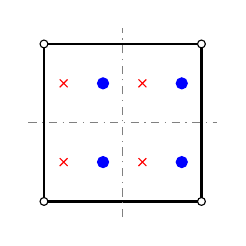
\begin{tikzpicture}[scale=1.]
    \draw[black,thick] (-1.,-1.) rectangle (1.,1.);
    \draw[black!50,dashdotted] (-1.2,0.) -- (1.2,0.0);\draw[black!50,dashdotted] (.0,-1.2) -- (0.,1.2);
    %% nodes
    \fill[white] (-1,-1) circle (0.05);\draw (-1,-1) circle (0.05);
    \fill[white] (1.,-1) circle (0.05);\draw (1,-1) circle (0.05);
    \fill[white] (1,1) circle (0.05);\draw (1,1) circle (0.05);
    \fill[white] (-1.,1) circle (0.05);\draw (-1,1) circle (0.05);
    %% particles
    \draw[Blue,mark=*] plot coordinates {(-0.5+0.25,-0.5)};
    \draw[Blue,mark=*] plot coordinates {(0.5+0.25,0.5)};
    \draw[Blue,mark=*] plot coordinates {(-0.5+0.25,0.5)};
    \draw[Blue,mark=*] plot coordinates {(0.5+0.25,-0.5)};
    \draw[Red,mark=x] plot coordinates {(-0.5-0.25,-0.5)};
    \draw[Red,mark=x] plot coordinates {(0.5-0.25,0.5)};
    \draw[Red,mark=x] plot coordinates {(-0.5-0.25,0.5)};
    \draw[Red,mark=x] plot coordinates {(0.5-0.25,-0.5)};
  \end{tikzpicture}  & 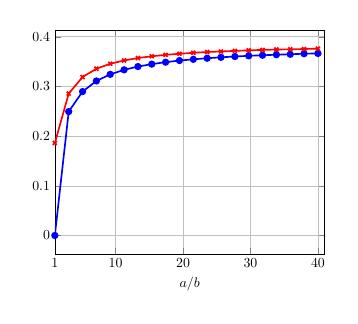
\begin{tikzpicture}[scale=0.5]
\begin{axis}[xlabel=$a/b$,ymajorgrids=true,xmajorgrids=true,xmin=1,xmax=41,xtick={1,10,20,30,40}]
%%%%%%%%%%% NATURAL CONFIGURATION
\addplot[Blue,mark=*,very thick] coordinates {(1.0,1.0000100001e-05) (3.05263157895,0.249310914162) (5.10526315789,0.28957342205) (7.15789473684,0.311013636452) (9.21052631579,0.324305874638) (11.2631578947,0.333392807612) (13.3157894737,0.339955504818) (15.3684210526,0.344870817129) (17.4210526316,0.348772961414) (19.4736842105,0.352087731404) (21.5263157895,0.354541966472) (23.5789473684,0.356753041215) (25.6315789474,0.358589375367) (27.6842105263,0.360175180699) (29.7368421053,0.361603616036) (31.7894736842,0.362721521952) (33.8421052632,0.363806269642) (35.8947368421,0.364694173258) (37.9473684211,0.365816289742) (40.0,0.366403664037) };
%%%%%%%%%%% MODIFIED CONFIGURATION
\addplot[Red,mark=x,very thick] coordinates {(1.0,0.186161861619) (3.05263157895,0.285515486734) (5.10526315789,0.318877925621) (7.15789473684,0.335565460918) (9.21052631579,0.345582403192) (11.2631578947,0.352315102098) (13.3157894737,0.357133045015) (15.3684210526,0.36070044911) (17.4210526316,0.363581004231) (19.4736842105,0.365719446668) (21.5263157895,0.367673150416) (23.5789473684,0.36925000829) (25.6315789474,0.37038001959) (27.6842105263,0.371525820521) (29.7368421053,0.372606357643) (31.7894736842,0.37353005109) (33.8421052632,0.374297427185) (35.8947368421,0.37474480008) (37.9473684211,0.375303226716) (40.0,0.376003760038) };
\end{axis}
\end{tikzpicture}
%%% Local Variables:
%%% mode: latex
%%% TeX-master: "../../mainManuscript"
%%% End:
 &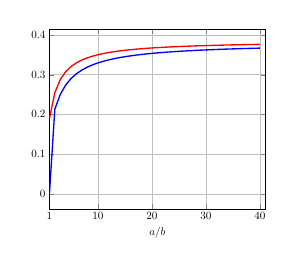
\begin{tikzpicture}[scale=0.4]
\begin{axis}[xlabel=$a/b$,ymajorgrids=true,xmajorgrids=true,xmin=1,xmax=41,xtick={1,10,20,30,40}]
%%%%%%%%%%% NATURAL CONFIGURATION
\addplot[Blue,very thick] coordinates {(1.0,-1.59364188514e-12) (2.0,0.212857320897) (3.0,0.249893924351) (4.0,0.27360416432) (5.0,0.290070593852) (6.0,0.30216822431) (7.0,0.311430129824) (8.0,0.318747857117) (9.0,0.324674954147) (10.0,0.329573175966) (11.0,0.333688883167) (12.0,0.337195633388) (13.0,0.340219213023) (14.0,0.342853009248) (15.0,0.345167807082) (16.0,0.347218235209) (17.0,0.349047125479) (18.0,0.350688533417) (19.0,0.352169876071) (20.0,0.3535134741) (21.0,0.354737683146) (22.0,0.355857736689) (23.0,0.356886382692) (24.0,0.357834370589) (25.0,0.358710828109) (26.0,0.359523555947) (27.0,0.360279260443) (28.0,0.360983738964) (29.0,0.361642028851) (30.0,0.362258527996) (31.0,0.362837093184) (32.0,0.36338112082) (33.0,0.363893613627) (34.0,0.364377236081) (35.0,0.364834360724) (36.0,0.365267107082) (37.0,0.365677374516) (38.0,0.36606687008) (39.0,0.366437132262) (40.0,0.366789551283) };
%%%%%%%%%%% MODIFIED CONFIGURATION
\addplot[Red,very thick] coordinates {(1.0,0.18887015067) (2.0,0.254459520239) (3.0,0.287403904864) (4.0,0.307169534548) (5.0,0.320334758075) (6.0,0.329729082668) (7.0,0.336768311765) (8.0,0.342238808871) (9.0,0.346612107914) (10.0,0.350188061313) (11.0,0.353166425063) (12.0,0.355685394958) (13.0,0.357843617559) (14.0,0.359713389803) (15.0,0.361348904135) (16.0,0.362791580609) (17.0,0.364073619671) (18.0,0.36522043174) (19.0,0.366252337065) (20.0,0.367185779335) (21.0,0.368034207917) (22.0,0.368808729666) (23.0,0.369518597597) (24.0,0.370171582133) (25.0,0.370774256583) (26.0,0.371332219112) (27.0,0.371850267081) (28.0,0.372332535292) (29.0,0.372782606539) (30.0,0.373203600747) (31.0,0.373598247379) (32.0,0.373968944663) (33.0,0.374317808349) (34.0,0.374646712123) (35.0,0.374957321245) (36.0,0.375251120754) (37.0,0.375529439201) (38.0,0.375793468735) (39.0,0.376044282167) (40.0,0.376282847537) };
\end{axis}
\end{tikzpicture}
%%% Local Variables:
%%% mode: latex
%%% TeX-master: "../../mainManuscript"
%%% End:
& \\ [3.25cm]
  %%%%%%%%%%%%%%%%%%%%%%%%%%%%%%%%%%%%%
  %%%%%%%%%%%%%%%%%%%%%%%%%%%%%%%%%%%%%
  \hline % Shifted above // Shifted below
  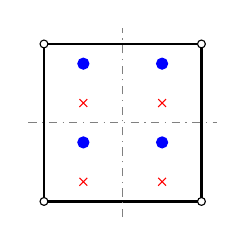
\begin{tikzpicture}[scale=1.]
    \draw[black,thick] (-1.,-1.) rectangle (1.,1.);
    \draw[black!50,dashdotted] (-1.2,0.) -- (1.2,0.0);\draw[black!50,dashdotted] (.0,-1.2) -- (0.,1.2);
    %% nodes
    \fill[white] (-1,-1) circle (0.05);\draw (-1,-1) circle (0.05);
    \fill[white] (1.,-1) circle (0.05);\draw (1,-1) circle (0.05);
    \fill[white] (1,1) circle (0.05);\draw (1,1) circle (0.05);
    \fill[white] (-1.,1) circle (0.05);\draw (-1,1) circle (0.05);
    %% particles
    \draw[Blue,mark=*] plot coordinates {(-0.5,-0.5+0.25)};
    \draw[Blue,mark=*] plot coordinates {(0.5,0.5+0.25)};
    \draw[Blue,mark=*] plot coordinates {(-0.5,0.5+0.25)};
    \draw[Blue,mark=*] plot coordinates {(0.5,-0.5+0.25)};
    \draw[Red,mark=x] plot coordinates {(-0.5,-0.5-0.25)};
    \draw[Red,mark=x] plot coordinates {(0.5,0.5-0.25)};
    \draw[Red,mark=x] plot coordinates {(-0.5,0.5-0.25)};
    \draw[Red,mark=x] plot coordinates {(0.5,-0.5-0.25)};
  \end{tikzpicture}& 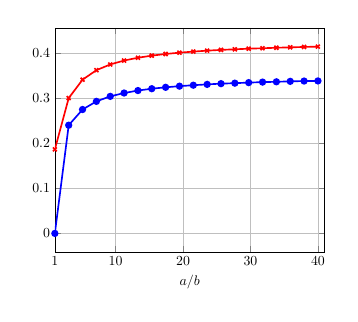
\begin{tikzpicture}[scale=0.5]
\begin{axis}[xlabel=$a/b$,ymajorgrids=true,xmajorgrids=true,xmin=1,xmax=41,xtick={1,10,20,30,40}]
%%%%%%%%%%% NATURAL CONFIGURATION
\addplot[Blue,mark=*,very thick] coordinates {(1.0,1.0000100001e-05) (3.05263157895,0.239878188256) (5.10526315789,0.274614851412) (7.15789473684,0.292689242682) (9.21052631579,0.303766195557) (11.2631578947,0.311204164673) (13.3157894737,0.316652640211) (15.3684210526,0.32074215479) (17.4210526316,0.323860607027) (19.4736842105,0.326382211191) (21.5263157895,0.328494863896) (23.5789473684,0.330344356075) (25.6315789474,0.331932266691) (27.6842105263,0.333044383075) (29.7368421053,0.334245447718) (31.7894736842,0.335382301191) (33.8421052632,0.336055465818) (35.8947368421,0.337054949497) (37.9473684211,0.337734956297) (40.0,0.338003380034) };
%%%%%%%%%%% MODIFIED CONFIGURATION
\addplot[Red,mark=x,very thick] coordinates {(1.0,0.186161861619) (3.05263157895,0.299954578493) (5.10526315789,0.340728670445) (7.15789473684,0.361763617636) (9.21052631579,0.374503745037) (11.2631578947,0.383176463344) (13.3157894737,0.389357577786) (15.3684210526,0.394050256292) (17.4210526316,0.397726608845) (19.4736842105,0.400577689987) (21.5263157895,0.402976661346) (23.5789473684,0.405090366693) (25.6315789474,0.406777225667) (27.6842105263,0.408069343851) (29.7368421053,0.409480410594) (31.7894736842,0.410406209325) (33.8421052632,0.411524115241) (35.8947368421,0.412434650662) (37.9473684211,0.413250974615) (40.0,0.414004140041) };
\end{axis}
\end{tikzpicture}
%%% Local Variables:
%%% mode: latex
%%% TeX-master: "../../mainManuscript"
%%% End:
 &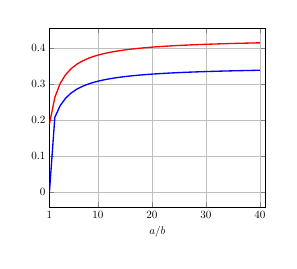
\begin{tikzpicture}[scale=0.4]
\begin{axis}[xlabel=$a/b$,ymajorgrids=true,xmajorgrids=true,xmin=1,xmax=41,xtick={1,10,20,30,40}]
%%%%%%%%%%% NATURAL CONFIGURATION
\addplot[Blue,very thick] coordinates {(1.0,-6.54115650537e-13) (2.0,0.207631685065) (3.0,0.240430029398) (4.0,0.26096289659) (5.0,0.275016910974) (6.0,0.285237324443) (7.0,0.293003101823) (8.0,0.299103117316) (9.0,0.304021109389) (10.0,0.308070133656) (11.0,0.311461709667) (12.0,0.314343883947) (13.0,0.316823369995) (14.0,0.318979027962) (15.0,0.320870393341) (16.0,0.322543253386) (17.0,0.324033398269) (18.0,0.325369207815) (19.0,0.326573474704) (20.0,0.327664714709) (21.0,0.328658124781) (22.0,0.329566294666) (23.0,0.330399742969) (24.0,0.331167326188) (25.0,0.331876554506) (26.0,0.332533838231) (27.0,0.33314468201) (28.0,0.333713839307) (29.0,0.334245436298) (30.0,0.334743072039) (31.0,0.335209900028) (32.0,0.335648695078) (33.0,0.336061908505) (34.0,0.336451713928) (35.0,0.336820045512) (36.0,0.337168630053) (37.0,0.337499014044) (38.0,0.337812586608) (39.0,0.33811059902) (40.0,0.338394181387) };
%%%%%%%%%%% MODIFIED CONFIGURATION
\addplot[Red,very thick] coordinates {(1.0,0.18887015067) (2.0,0.262956392078) (3.0,0.302076047328) (4.0,0.32618849157) (5.0,0.342522128096) (6.0,0.354312580524) (7.0,0.363221663933) (8.0,0.370189579051) (9.0,0.375787926093) (10.0,0.380384094421) (11.0,0.384224929247) (12.0,0.387482399219) (13.0,0.390279973956) (14.0,0.392708588922) (15.0,0.394836695539) (16.0,0.396716803678) (17.0,0.398389865869) (18.0,0.399888290415) (19.0,0.401238058753) (20.0,0.402460243029) (21.0,0.403572113124) (22.0,0.404587957102) (23.0,0.405519698035) (24.0,0.406377363812) (25.0,0.407169449254) (26.0,0.407903198264) (27.0,0.408584825881) (28.0,0.409219694664) (29.0,0.409812455992) (30.0,0.410367164166) (31.0,0.41088736923) (32.0,0.411376192992) (33.0,0.411836391706) (34.0,0.412270408049) (35.0,0.412680414481) (36.0,0.413068349603) (37.0,0.413435948794) (38.0,0.413784770166) (39.0,0.414116216626) (40.0,0.414431554738) };
\end{axis}
\end{tikzpicture}
%%% Local Variables:
%%% mode: latex
%%% TeX-master: "../../mainManuscript"
%%% End:
& \\ [3.25cm]
  %\begin{minipage}{0.85\textwidth}\lipsum[1]\end{minipage}
  \hline
\end{tabular}

%%% Local Variables: 
%%% mode: latex
%%% TeX-master: "../../mainManuscript"
%%% End:
  \caption{Values of critical Courant number $a\frac{\Delta t}{\Delta X}$ for two-dimensional DGMPM scheme using either DCU or CTU with respect to the material points distribution as a function of the speeds ratio $a/b$.}
  \label{tab:2DCFL_comparison_4ppc}
\end{table}


%Before concluding this chapter, some differences between the stability properties of DGMPM and MPM schemes are emphasized. First, the one and two-dimensional scheme equations written for the DGMPM enable, through the linear von Neumann stability analysis, the computation of 
%The von Neumann linear stability analysis performed in this section provides an explicit (nonlinear) condition \eqref{eq:stability} that must be satisfied in order to ensure the stability of DGMPM schemes. First, this relation allows to fully exploit the ability of the method to rebuild the grid mesh arbitrarily. Indeed, after such a procedure, the number and positions of material points in grid cells can change and one must be able to adapt properly the CFL number so that the scheme remains stable. An advantage on the original MPM is hence highlighted since no stability condition exists for the method. Second, it has been shown that some DGMPM discretizations provide an improvement of the restrictive CFL number that applies to the DGFEM scheme. In particular, the optimal condition allowing to capture discontinuities ($CFL=1$) can be achieved for several space-time discretizations. This property turns out to be a strength for the DGMPM since it aims at follow waves accurately.

%One can imagine to place material points so that an optimal stability condition is reached by minimizing some functional constrained with the description of material boundaries.

%%% Local Variables: 
%%% mode: latex
%%% TeX-master: "../mainManuscript"
%%% End:
